\documentclass[lettersize,journal]{IEEEtran}

% Language setting Replace `english' with e.g. `spanish' to change the document
% language
\usepackage[english]{babel}
\usepackage{caption}
\usepackage{subcaption}
\usepackage{makecell}
% \usepackage[toc,page]{appendix}
\setlength{\marginparwidth}{2cm}
\usepackage{todonotes}
\usepackage{soul}
\usepackage{pdflscape}

% Set page size and margins Replace `letterpaper' with `a4paper' for UK/EU
% standard size
\usepackage[letterpaper,top=2cm,bottom=2cm,left=3cm,right=3cm,marginparwidth=1.75cm]{geometry}

% Useful packages
\usepackage{amsmath}
\usepackage{amsfonts}
\usepackage{amssymb}
\usepackage{graphicx}
\usepackage{xspace}
\usepackage{xcolor}% http://ctan.org/pkg/xcolor
\usepackage{hyperref}
\usepackage{colortbl}
\usepackage{dsfont}

\setlength{\marginparwidth}{2cm}
\usepackage{todonotes}
\usepackage{etoolbox}
\usepackage{xargs}
\usepackage{multirow}

% Fix link colors
\hypersetup{
    colorlinks = true,
    linkcolor=red,
    citecolor=red,
    urlcolor=blue,
    linktocpage % so that page numbers are clickable in toc
}

\newcommand{\TODO}[1]{\color{red}\textsc{TODO:} #1\color{black}\xspace}
\newcommand{\TG}[1]{\color{orange}\textsc{From Tristan:} #1\color{black}\xspace}
\newcommand{\fmriprep}{fMRIPrep\xspace}
\newcommand{\fwhm}{\textsc{FWHM}}

\newcommand{\failcolor}{orange} % HEX #009E73
\newcommand{\passcolor}{green} % HEX #D55E00

\hyphenation{pre-processing}


\newcommand\Mark[2][8.4]{%
  \rlap{\tikz[baseline=(current bounding box.south)]{
        \shade[left color=\color{red}, right color=\color{green}, middle color=\color{yellow}]
               (0,0) rectangle ++(#1*#2/100,0.3);}%
  }%
}

\newtoggle{RRandRS}
\togglefalse{RRandRS} % Set it to true or false based on your requirement


\newlength{\figureWidthUM}
\newlength{\vspaceIndex}

\newcommandx{\uncertaintyMap}[5][5=false]{%
  % arguments:
  % 1: FWHM 
  % 2: subject index
  % 3: dataset
  % 4: subject
  % 5: add columns title
%   \iftoggle{RRandRS}{\setlength{\figureWidthUM}{0.2\paperheight}}{\setlength{\figureWidthUM}{0.27\paperheight}}
  \setlength{\figureWidthUM}{0.15\paperheight}
  \ifstrequal{#5}{true}{\setlength{\vspaceIndex}{-45pt}}{\setlength{\vspaceIndex}{25pt}}
  \begin{subfigure}[b]{0.01\paperwidth}
    \centering
    #2\vspace*{\vspaceIndex}
  \end{subfigure}
  \begin{subfigure}[t]{\figureWidthUM}
    \centering
    \ifstrequal{#5}{true}{IEEE (T1 intensity)}{}
    \includegraphics[width=\textwidth]{figures/sig/#1mm/ieee_#3_#4.pdf}
  \end{subfigure}
  \begin{subfigure}[t]{\figureWidthUM}
    \centering
    \ifstrequal{#5}{true}{RR (significant bits)}{}
    \includegraphics[width=\textwidth]{figures/sig/#1mm/rr_#3_#4_sig.pdf}
  \end{subfigure}
  \begin{subfigure}[t]{\figureWidthUM}
    \centering
    \ifstrequal{#5}{true}{RS (significant bits)}{}
    \includegraphics[width=\textwidth]{figures/sig/#1mm/rs_#3_#4_sig.pdf}
  \end{subfigure}
  \iftoggle{RRandRS}{%
    \begin{subfigure}[t]{\figureWidthUM}
      \centering
      \ifstrequal{#5}{true}{RR+RS (significant bits)}{}
      \includegraphics[width=\textwidth]{figures/sig/#1mm/rr.rs_#3_#4_sig.pdf}
    \end{subfigure}
  }{}
}

\newcommandx{\uncertaintyMapDiscrete}[5][5=false]{%
  % arguments:
  % 1: FWHM 
  % 2: subject index
  % 3: dataset
  % 4: subject
  % 5: add columns title
%   \iftoggle{RRandRS}{\setlength{\figureWidthUM}{0.2\paperheight}}{\setlength{\figureWidthUM}{0.27\paperheight}}
  \setlength{\figureWidthUM}{0.15\paperheight}
  \ifstrequal{#5}{true}{\setlength{\vspaceIndex}{-45pt}}{\setlength{\vspaceIndex}{25pt}}
  \begin{subfigure}[b]{0.01\paperwidth}
    \centering
    #2\vspace*{\vspaceIndex}
  \end{subfigure}
  \begin{subfigure}[t]{\figureWidthUM}
    \centering
    \ifstrequal{#5}{true}{IEEE (T1 intensity)}{}
    \includegraphics[width=\textwidth]{figures/sig/#1mm/ieee_#3_#4.pdf}
  \end{subfigure}
  \begin{subfigure}[t]{\figureWidthUM}
    \centering
    \ifstrequal{#5}{true}{RR (significant bits)}{}
    \includegraphics[width=\textwidth]{figures/sig/discrete/#1mm/rr_#3_#4_sig_discrete.pdf}
  \end{subfigure}
  \begin{subfigure}[t]{\figureWidthUM}
    \centering
    \ifstrequal{#5}{true}{RS (significant bits)}{}
    \includegraphics[width=\textwidth]{figures/sig/discrete/#1mm/rs_#3_#4_sig_discrete.pdf}
  \end{subfigure}
  \iftoggle{RRandRS}{%
    \begin{subfigure}[t]{\figureWidthUM}
      \centering
      \ifstrequal{#5}{true}{RR+RS (significant bits)}{}
      \includegraphics[width=\textwidth]{figures/sig/discrete/#1mm/rr.rs_#3_#4_sig_discrete.pdf}
    \end{subfigure}
  }{}
}


% Cluster failure: Why fMRI inferences for spatial extent lhave inflated
% false-positive https://www.pnas.org/doi/pdf/10.1073/pnas.1602413113

\title{A numerical variability approach to results stability tests and its application to neuroimaging}
\author{\IEEEauthorblockN{Yohan Chatelain\IEEEauthorrefmark{1}, Loic Tetrel\IEEEauthorrefmark{2}, Christopher J. Markiewicz\IEEEauthorrefmark{3}, Gregory Kiar\IEEEauthorrefmark{6},\\ Oscar Esteban\IEEEauthorrefmark{3}\IEEEauthorrefmark{5},  Pierre Bellec\IEEEauthorrefmark{2}\IEEEauthorrefmark{4}, Tristan Glatard\IEEEauthorrefmark{1}\vspace*{0.2cm}}

\IEEEauthorblockA{\IEEEauthorrefmark{1}Department of Computer Science and Software Engineering\\ Concordia University, Montreal, Quebec, Canada.}

\IEEEauthorblockA{\IEEEauthorrefmark{2} Centre de recherche de l'Institut Universitaire de Gériatrie\\ de Montréal (CRIUGM), Montréal, Québec, Canada.}

\IEEEauthorblockA{\IEEEauthorrefmark{3} Department of Psychology, Stanford University, Stanford, CA, USA.}

\IEEEauthorblockA{\IEEEauthorrefmark{4} Department of Psychology, Université de Montréal, Montréal, Québec, Canada.}

\IEEEauthorblockA{\IEEEauthorrefmark{5} Department of Radiology, Lausanne University Hospital\\ and University of Lausanne, Switzerland.}

\IEEEauthorblockA{\IEEEauthorrefmark{6} Child Mind Institute, New York City, NY, USA.}
}



\begin{document}
\maketitle

\begin{abstract}
    Ensuring the long-term reproducibility of data analyses requires results stability tests to ensure that analysis results remain within acceptable variation bounds despite inevitable software updates and hardware evolutions. This paper introduces a numerical variability approach for results stability tests, which determines acceptable variation bounds using random rounding of floating-point calculations. By applying the resulting stability test to \fmriprep, a widely-used neuroimaging tool, we show that the test is sensitive enough to detect subtle updates in image processing methods while remaining specific enough to be tolerant to numerical variations within a reference version of the application. This result contributes to enhancing the reliability and reproducibility of data analyses by providing a robust and flexible method for stability testing.
\end{abstract}

\section{Introduction}

% results stability tests
Data analyses can produce different results depending on the hardware and software conditions in which they are executed~\cite{gronenschild2012effects}, which has important repercussions in a number of disciplines. This paper investigates results stability tests whereby the outcome of a data analysis is asserted to remain within acceptable variation bounds of a reference result. The primary challenge in developing such stability tests lies in the determination of acceptable bounds of variation around the reference result. We define such bounds from the numerical variability of the results, that is, from the variability inherent to numerical computations.

% neuroimaging
We focus on the use case of neuroimaging analyses, although our method applies to data analyses more broadly. For several decades, the neuroimaging community has developed advanced software tools enabling researchers to study the human brain with unprecedented detail and precision. Neuroimaging tools now underpin scientific findings in several disciplines, and must therefore be thoroughly tested. In particular, neuroimaging studies often follow subjects over multiple years, which requires data analyses to be consistent over substantial time periods.


% fmriprep
The present paper focuses primarily on the \fmriprep software~\cite{esteban2019fmriprep}, a tool to pre-process Magnetic Resonance Imaging (MRI) data as a pre-requisite of any further analysis. \fmriprep is an integrated data analysis pipeline for structural and functional MRI pre-processing. We focus on the pre-processing of structural MRI, which includes intensity non-uniformity correction, skull stripping, and spatial normalization to a brain template. 
%Spatial normalization is a critical step of MRI analysis whereby images acquired on individual subjects are mapped to a template brain through a process called image registration. 
 \fmriprep developers recently initiated long-term support (LTS) releases to guarantee results stability over multiple years, which motivated the development of the results stability tests presented in this paper. 

% is challenging due to inevitable security updates and bug fixes in the main software or in its dependencies.

% numerical precision
Our stability tests leverage the numerical variability resulting from the use of finite-precision arithmetic in calculations. This variability manifests primarily as a result of changes in  computational environments, which includes hardware architecture, parallelization scheme, operating system, and software dependencies. To estimate numerical variability, we rely on random rounding~\cite{forsythe1959reprint}, a stochastic arithmetic technique that randomly rounds floating-point operation results to the previous or to the next floating-point number. Stochastic arithmetic has been successfully applied to simulate numerical variability in various domains, including neuroimaging~\cite{salari2021accurate, kiar2021numerical}. Our approach is not specific to any particular numerical scheme and relies on a few statistical assumptions such as normality and independence, making it applicable to a wide range of scenarios.

% summary of contributions
In summary, the main contributions of this paper are (1) the introduction of a numerical variability approach to results stability tests, (2) the construction of results stability tests for structural pre-processing in \fmriprep, and (3) the evaluation of the resulting stability tests in a number of configurations.

\section{Results stability test design}

Considering a data processing application $\Lambda$, the objective of our stability test is to determine whether the results generated by a different application $\tilde \Lambda$ significantly differ from the reference results produced by $\Lambda$. In practice, we are particularly interested in the case where $\tilde \Lambda$ corresponds to a different version of $\Lambda$, or to the same version executed in a different execution environment (operating system, parallelization or hardware). Given input data $I$, we assume that $\Lambda$ and $\tilde \Lambda$ produce images $X$ and $\tilde X$ with the same number $v$ of voxels. We model $X$ as a random variable and we sample its distribution by computing $n$ random numerical perturbations of $\Lambda$, resulting in $n$ images $X_k$. Conversely, we compute $\tilde X$ without random perturbation using the IEEE-754 norm, to avoid computational overheads at test time. To test if $\tilde X$ belongs to the distribution of $X$, we perform a z-test for each voxel $\tilde x_i$ ($i\leq v$), using the mean $\hat \mu_i$ and the standard deviation $\hat \sigma_i$ estimated from the $n$ perturbed results. The test computes a p-value $p_i$ under the null hypothesis $H_{0,i}$ that the tested voxel belongs to the reference distribution:
\begin{equation} \label{eq:pval}
    p_i(z_i) = 2 \left(1-\Phi(z_i)\right),
\end{equation}
where $\Phi$ is the cumulative distribution function of the normal centered
Gaussian and:
\begin{equation*}
    z_i = \frac{\tilde x_i-\hat \mu_i}{\hat \sigma_i},
\end{equation*}
where $\tilde x_i$ is the intensity of a voxel in $\tilde X$, $v$ is the number of voxels in $\tilde X$, and $\hat \mu_i$ and $\hat \sigma_i$ are the mean and standard deviation voxel intensities estimated from the $n$ perturbed results $X_k$. $H_{0,i}$ is rejected when $p_i$ is lower than a threshold $\alpha$ that also defines the confidence level of the test (1-$\alpha$)\%. The z-test assumes that perturbed voxel intensities are normally distributed. To capture anatomical variability, we perform this test on a representative set of input images described hereafter. Table~\ref{tab:notations} summarizes the notations and Figure~\ref{fig:test_workflow} summarizes the test workflow.

\begin{figure}
    \centering
    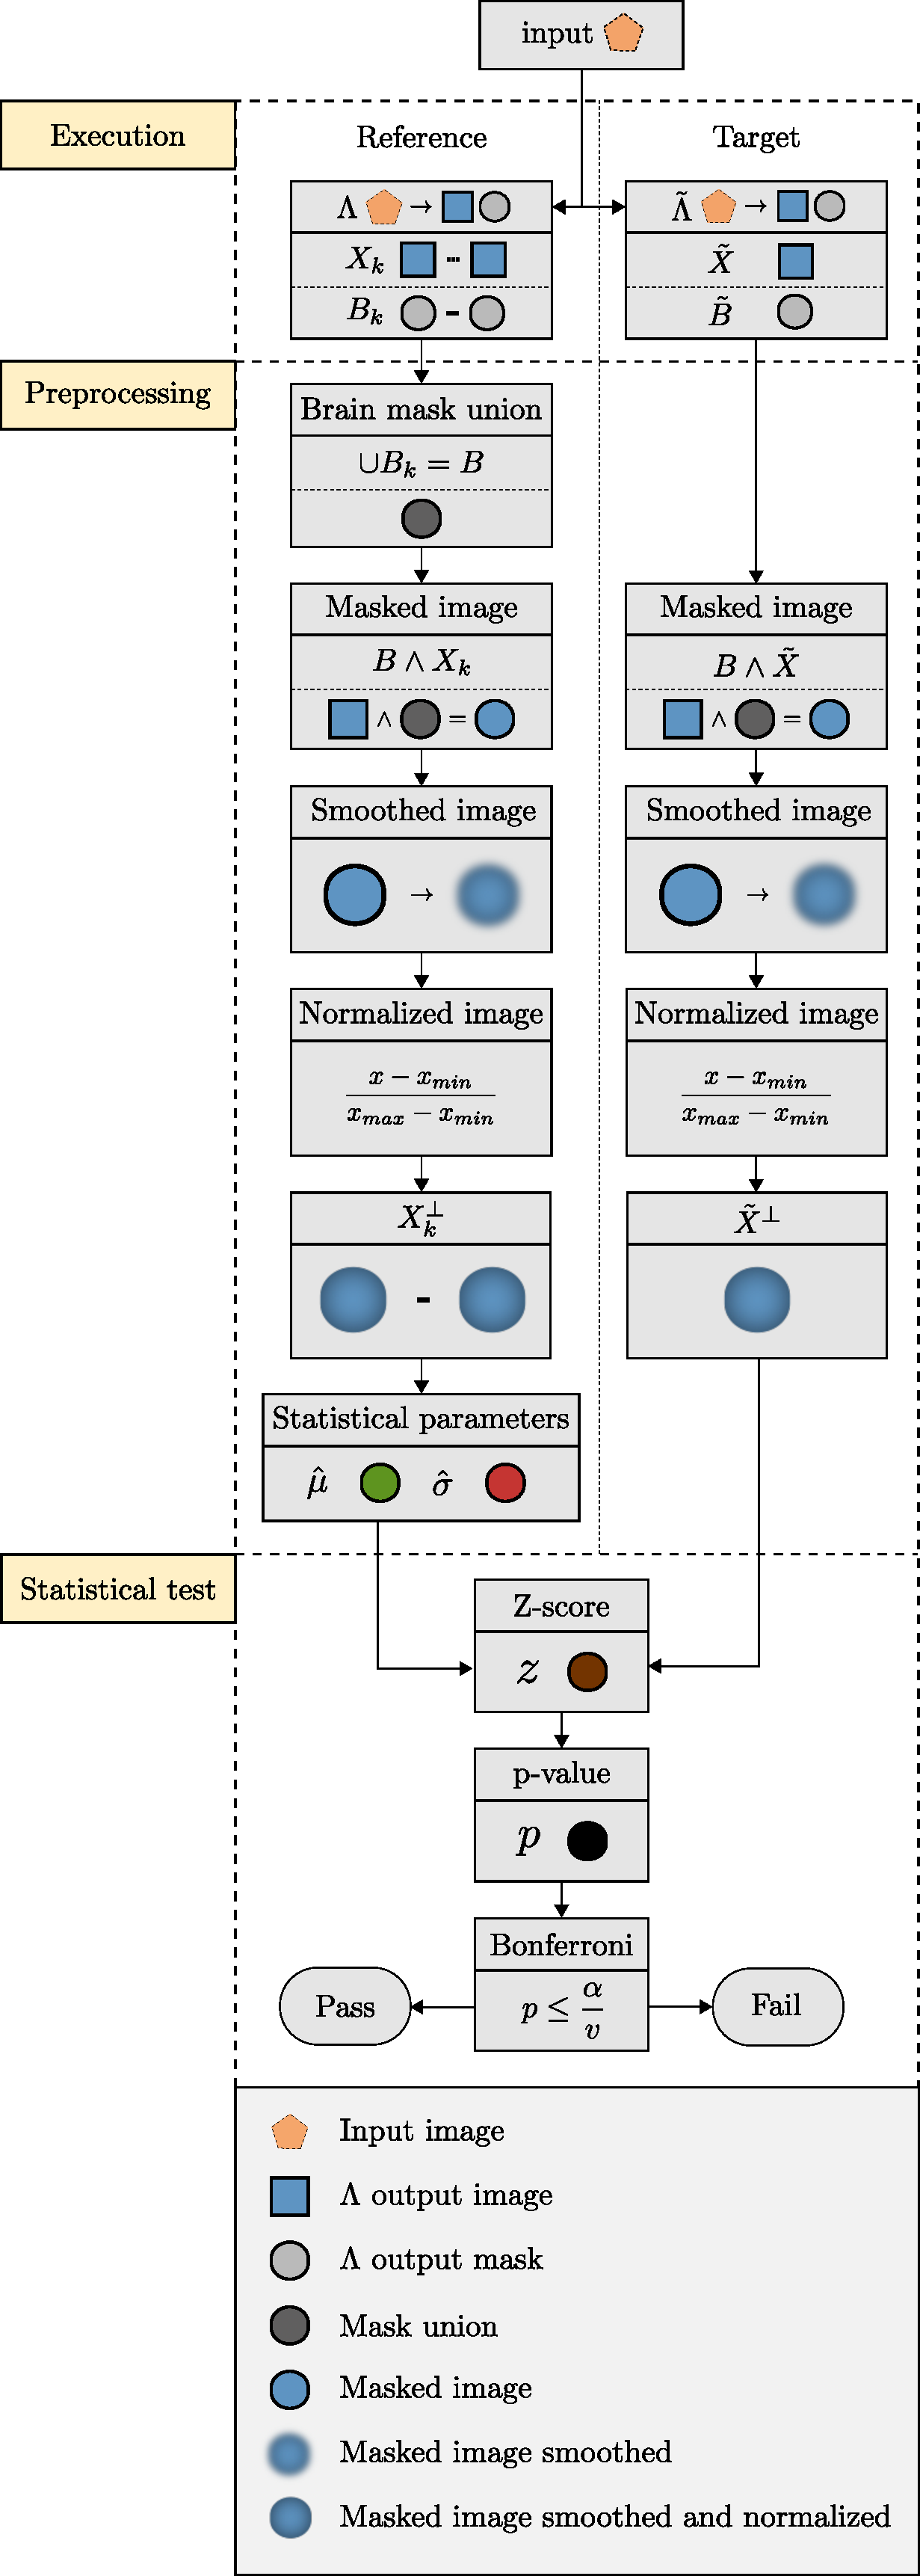
\includegraphics[width=\columnwidth]{figures/workflow_V.pdf}
    \caption{Stability test construction and evaluation. The reference application $\Lambda$ is executed $n$ times on the input data, with random perturbations, resulting in images $X_k$ from which a null distribution is built to test the result produced by target application $\tilde \Lambda$. All results undergo the same smoothing and normalization steps. \TG{in masked images: the pictograms are not in the same order as the letters. I'm not sure why the normalization is split in two boxes. Add some whitespace between the workflow and the caption.}}
    \label{fig:test_workflow}
\end{figure}
\begin{table}
    \centering
    \begin{tabular}{r|l}
        $\Lambda$          & reference application                                                \\
        $\tilde \Lambda$   & tested application                                                   \\
        $i$                & index of a voxel in the brain mask                                   \\
        $v$                & number of voxels in the brain mask                                   \\
        $k$                & index of a perturbed sample                                          \\
        $n$                & number of perturbed samples                                          \\
        $\tilde x_i$       & voxel intensity in image $\tilde X$                                  \\
        $z_i$              & z-score of voxel i                                                   \\
        $p_i$              & p-value of voxel i                                                   \\
        $\hat{\mu_i}$      & average voxel intensity across perturbed samples                     \\
        $\hat{\sigma_i}$   & standard deviation of voxel intensity across perturbed\\ & samples       \\
        $B_k$              & brain masks produced by random numerical \\ & perturbations of $\Lambda$  \\
        $B$                & union of $B_k$ masks                                                 \\
        $\tilde X$         & image produced by unperturbed $\tilde \Lambda$ using IEEE \\ & convention \\
        $X_k$              & images produced by random numerical perturbations \\ & of $\Lambda$       \\
        $X_k^{\perp}$      & $X_k$ masked with $B$, min-max scaled and spatially \\ & smoothed         \\
        $\hat{s}$          & average number of significant bits across the image                  \\
        $\mathcal{N}(0,1)$ & standard Gaussian distribution                                       \\
        $\Phi$             & cumulative distribution function of $\mathcal{N}(0,1)$               \\
        $\chi^2_{n-1}$     & Chi-2 distribution with n-1 degrees of freedom                       \\
    \end{tabular}
    \caption{Notations}
    \label{tab:notations}
\end{table}


\subsection{Numerical variability estimation}

To estimate the distribution of reference results and compute $\hat \mu_i$ and $\hat \sigma_i$, we sample results distributions by applying two types of random numerical perturbations: (1) Random Rounding (RR), which randomly rounds function outputs in the GNU libmath mathematical library, and (2) Random Seed (RS), which varies the random seed used in the application. In neuroimaging, random seeds are typically employed to initialize optimization processes encountered in spatial normalization.

Random Rounding (RR) consists in rounding the exact result of a floating-point arithmetic operation toward the previous or next floating-point number~\cite{forsythe1959reprint}. RR is equivalent to applying Monte-Carlo Arithmetic (MCA~\cite{parker1997monte}) to double-precision numbers with a virtual precision of 53 bits and to single-precision numbers with a virtual precision of 24 bits, which was shown to accurately simulate the effect of operating system updates on the structural MRI pre-processing pipelines of the Human Connectome Project (HCP) when applied to GNU libmath~\cite{salari2021accurate}. Structural HCP pipelines consist of tools assembled from the FSL~\cite{jenkinson2012fsl} and Freesurfer~\cite{fischl2012freesurfer} toolboxes, which makes them conceptually very similar to the structural fMRIPrep pipeline targeted by our study.

RR is rigorously implemented in several tools including CADNA~\cite{jezequel2008cadna}, Verrou~\cite{fevotte2016verrou}, and Verificarlo~\cite{denis2016verificarlo}. However, these tools incur substantial performance overheads which makes them hard to apply to compute-intensive applications. In addition, only Verrou supports RR instrumentation of GNU libmath~\cite{fevotte2019debugging}, and it does so by relying on quadruple precision, which is not scalable to entire neuroimaging pipelines. Therefore, we implemented a fast, approximate RR method by randomly adding or removing 1 ulp (unit in the last place) to the outputs of GNU libmath functions. Our implementation, available on GitHub (\url{https://github.com/verificarlo/fuzzy/blob/master/docker/resources/libmath/fast/src/wrapping\_script.c}),  only approximates RR as it applies a random perturbation to an already rounded result instead of to the exact result as done in rigorous implementations. In practice, computing the exact result returned by GNU libmath functions, by using MPFR~\cite{fousse2007mpfr} for instance, is too expensive for our use case.

Random Seed (RS) and RR trigger different types of variability. RR can be applied transparently to any application while RS is more specific to the type of analysis. Conversely, RR incurs a substantial performance overhead whereas RS does not.

\subsection{fMRIprep results preprocessing}

For the \fmriprep application, $X_k$ is the main structural derivative produced by \fmriprep, that is, the T1-weighted MRI image corrected for intensity non-uniformity using \texttt{N4BiasFieldCorrection} from \texttt{ANTS} and transformed to template space using \texttt{antsRegistration}. This file is named \texttt{desc-preproc\_T1w} in the \fmriprep outputs. In addition to $X_k$, \fmriprep produces a brain mask $B_k$, a segmentation into grey matter, white matter and cerebrospinal fluid tissues, as well as probability maps for each of these tissues.

Before computing the p-values in Equation~\ref{eq:pval}, we apply brain masking, smoothing, and intensity normalization to $X_k$. For brain masking, we mask $X_k$ with the union of the brain masks produced across all perturbed results. We use the union of the brain masks rather than their intersection to capture variability across $B_k$ masks. For smoothing, we apply a spatial 3D Gaussian smoothing kernel with Full-Width at Half Maximum (\fwhm) ranging from 0mm to 20mm. For intensity normalization, we apply a min-max scaling to the smoothed intensities to scale them to [0,1].
The resulting pre-processed image $X_k^\perp$ is used as input of the stability test.

\subsection{Datasets}

We selected eight test subjects from sub-datasets in the OpenNeuro~\cite{markiewicz2021openneuro} data-sharing platform, representing a diversity of ages, sex, and study designs. The datasets include a motion study with children (ds000256), a long-term memory study with young adults (ds001748), and a motor process study with adults (ds002338). In addition, two sub-datasets involve steps of the pipeline that can affect its reproducibility, namely different field maps (ds001600) and non-structural images (ds001771). Table~\ref{table:dataset_info} lists the dimension, voxels resolution, age and sex of each subject in the dataset.

\begin{table*}
    \begin{center}
        \begin{tabular}{c|c|l|c|c|c|c|c}
            Index & Dataset  & Subject     & Dimension ($x,y,z$)         & Voxel resolution            & Data type & Age     & Sex \\
                  &          &             &                             & $mm^3$ ($x,y,z$)            &           & (years) &     \\
            \hline
            1     & ds000256 & sub-CTS201  & $256 \times 256 \times 256$ & $1.0 \times 1.0 \times 1.0$ & int16     & 8.68    & M   \\
            2     & ds000256 & sub-CTS210  & $224 \times 256 \times 256$ & $0.8 \times 0.8 \times 0.8$ & int16     & 7.63    & F   \\
            3     & ds001600 & sub-1       & $176 \times 256 \times 256$ & $1.0 \times 1.0 \times 1.0$ & int16     & -       & -   \\
            4     & ds001748 & sub-adult15 & $176 \times 240 \times 256$ & $1.0 \times 1.0 \times 1.0$ & float32   & 21      & M   \\
            5     & ds001748 & sub-adult16 & $176 \times 240 \times 256$ & $1.0 \times 1.0 \times 1.0$ & float32   & 21      & F   \\
            6     & ds001771 & sub-36      & $256 \times 320 \times 320$ & $0.8 \times 0.8 \times 0.8$ & int16     & 22      & F   \\
            7     & ds002338 & sub-xp201   & $176 \times 512 \times 512$ & $1.0 \times 0.5 \times 0.5$ & int16     & 41      & F   \\
            8     & ds002338 & sub-xp207   & $176 \times 512 \times 512$ & $1.0 \times 0.5 \times 0.5$ & int16     & 39      & M   \\
        \end{tabular}
    \end{center}
    \caption{Dimension, voxels resolutions, age and sex of each subject in the dataset.}
    \label{table:dataset_info}
\end{table*}

\subsection{Handling multiple comparisons}

Handling multiple comparisons is a critical component of statistical testing in neuroimaging given the high number of voxels tested for each 3D structural image---typically more than 10 million~\cite{NICHOLS2007246}. The stability test defined in Equation~\ref{eq:pval} consists of independent z-tests performed for each of the $v$ voxels of each test image, resulting in a set of $v$ p-values $p_i$, $i \leq v$. We corrected for multiple comparisons by adjusting the p-value threshold using the classical Bonferroni correction that simply divides $\alpha$ by the number of multiple comparisons performed. As a result, the tested \fmriprep result is considered part of the reference distribution iff:
\begin{equation}
    \label{eq:bonferroni}
    \forall i \leq v, \quad p_i \geq \frac{\alpha}{v}.
\end{equation}

\subsection{Numerical stability measure}

As a by-product of test construction, we can measure numerical variability in the application results, which provides valuable information about their numerical quality.
We quantify numerical stability for each voxel using the number of significant bits, a metric to identify the bits containing signal from those containing only noise. We compute the number of significant bits $\hat{s}$ with probability $p_s=0.95$ and confidence $1-\alpha_s=0.95$ using the \texttt{significant\_digits} package v0.1.2 available at \url{https://github.com/verificarlo/significantdigits} that implements the Centered Normality Hypothesis approach described in~\cite{sohier2021confidence}:

\[
    \hat{s_i} = -\log_2 \left| \frac{\hat{\sigma_i}}{\hat{\mu_i}} \right| - \delta(n, \alpha_s, p_s)
\]
where $\hat{\sigma_i}$ and $\hat{\mu_i}$ are the voxelwise average and standard deviation over the $X_k^\perp$ perturbed results ($k \leq n$), and
\begin{equation}
    \begin{split}
        \delta(n, \alpha_s, p_s) =& \frac{1}{2} \left[ \log_2 \left( \frac{n-1}{\chi^2_{1-\alpha_s/2}} \right) + \right. \\
            &  \left. \log_2 \left( \Phi^{-1} \left( \frac{p_s+1}{2} \right) \right) \right]
    \end{split}
\end{equation}
is a penalty term to estimate $\hat{s_i}$ with probability $p_s$ and confidence level $1-\alpha_s$ for a sample size $n$. $\Phi^{-1}$ is the inverse cumulative distribution of the standard normal distribution and $\chi^2$ is the Chi-2 distribution with n-1 degrees of freedom.



\subsection{Computing infrastructure}

We processed the dataset using the Narval cluster managed by Calcul Qu\'ebec and part of the Digital Research Alliance of Canada. With our job submission parameters, we could access 1,145 computing nodes with 64 cores per node and 2 $\times$ AMD Rome 7532 @ 2.40 GHz 256M cache L3. We executed \fmriprep in a Singularity container built from a Docker image available on DockerHub \texttt{yohanchatelain/fmriprep-fuzzy:20.2.1}. The container image used Ubuntu \texttt{16.04.6 LTS}, GNU libc/libmath \texttt{2.23}, kernel \texttt{4.18.0-372.19.1}\texttt{.el8\_6.x86\_64}, and fMRIPrep version \texttt{20.2.1}. We disabled multi-threading in fMRIPrep, fixed the random seed for skull stripping as well as in fMRIPrep (RR condition only), and verified that in these conditions fMRIPrep results were bit-to-bit reproducible.
We used Fuzzy \texttt{v0.9.1-a} built with Verificarlo version \texttt{v0.9.1}. \TG{Here you should add a link to the github repo containing the notebooks to reproduce the results figures.}

\section{Results}

We computed n=30 perturbed results for each of the 8 subjects and for the two types of perturbations RR and RS. For RS, we used \fmriprep's command-line interface to set the random seed in all the pipeline components. We also computed an unperturbed IEEE result for each subject using the random seed used in RR (42). For each type of perturbation, we measured the numerical stability of fMRIPrep in terms of significant bits, and we built the stability test using different sizes of smoothing kernel and different confidence levels.

\subsection{Measured numerical variability was high and it varied across subjects}

\begin{figure}
    \centering
    \includegraphics[width=\linewidth]{figures/stats.pdf}
    \caption{Voxel-wise means of significant bits
        measured across n=30 perturbed samples for RR and RS perturbations and 8
        subjects. \TG{show the min y-value on this graph (is it 2 bits?)}}
    \label{fig:significant-digits}
\end{figure}
Overall, the two types of perturbations (RR and RS) resulted in numerical uncertainties of comparable magnitude and behavior (Figure~\ref{fig:significant-digits}), which supports the validity of our results. The measured numerical variability was high, with mean significant bits ranging from 2 bits to 10 bits out of the 12 bits available in the data\footnote{The voxel intensity is encoded on 12 bits although it is embedded in a 16 bits format.}. Numerically, the application appears to be highly sensitive to numerical and random seed perturbations.

We noted substantial discrepancies in numerical stability across subjects. For a given smoothing kernel size, the number of significant bits frequently varied in the ratio of 1 to 3 across subjects. Overall, smoothing tended to reduce numerical variability, however, this behavior was in general not monotonous and impacted subjects differently. The observed between-subject variability
demonstrates the importance of evaluating such applications on a representative set of datasets.

The numerical variability measured across perturbed samples showed regional variations compatible with anatomical features (Figure~\ref{fig:uncertainty-maps} and Appendix~\ref{appendix:numerical_uncertainty}). In particular, variability was
maximal at the border of the brain mask, and it was overall higher in the gray matter than in the white matter.
This is consistent with previous observations of numerical variability in structural brain image analysis~\cite{salari2021accurate}.
In addition, numerical variability was also maximal in some focal regions, suggesting that spatial normalization may be unstable in these regions. Our stability test will therefore be more tolerant in these regions.


% \begin{figure*}
%     \centering
%     \uncertaintyMap{15}{1}{ds000256}{sub-CTS201}[true] \\
%     \uncertaintyMap{15}{2}{ds000256}{sub-CTS210} \\
%     \uncertaintyMap{15}{3}{ds001600}{sub-1} \\
%     \uncertaintyMap{15}{4}{ds001748}{sub-adult15} \\
%     \uncertaintyMap{15}{5}{ds001748}{sub-adult16} \\
%     \uncertaintyMap{15}{6}{ds001771}{sub-36} \\
%     \uncertaintyMap{15}{7}{ds002338}{sub-xp201} \\
%     \uncertaintyMap{15}{8}{ds002338}{sub-xp207} \\
%     \includegraphics*[width=.6\linewidth]{figures/colorbar_sigbit.pdf}
%     \caption{Uncertainty measured for subjects 1 to 8 (from top to bottom) across n=30 perturbed samples, with FWHM=15mm. Uncertainty maps for other smoothing kernel sizes are available in Appendix~\ref{appendix:numerical_uncertainty}.}
%     \label{fig:uncertainty-maps}
% \end{figure*}

\begin{figure*}
    \centering
    \uncertaintyMapDiscrete{15}{1}{ds000256}{sub-CTS201}[true] \\
    \uncertaintyMapDiscrete{15}{2}{ds000256}{sub-CTS210} \\
    \uncertaintyMapDiscrete{15}{3}{ds001600}{sub-1} \\
    \uncertaintyMapDiscrete{15}{4}{ds001748}{sub-adult15} \\
    \uncertaintyMapDiscrete{15}{5}{ds001748}{sub-adult16} \\
    \uncertaintyMapDiscrete{15}{6}{ds001771}{sub-36} \\
    \uncertaintyMapDiscrete{15}{7}{ds002338}{sub-xp201} \\
    \uncertaintyMapDiscrete{15}{8}{ds002338}{sub-xp207} \\
    \includegraphics*[width=.6\linewidth]{figures/colorbar_sigbit_discrete.pdf}
    \caption{Numerical variability measured for subjects 1 to 8 (from top to bottom) across n=30 perturbed samples, with FWHM=15mm. Uncertainty maps for other smoothing kernel sizes are available in Appendix~\ref{appendix:numerical_uncertainty}.}
    \label{fig:uncertainty-maps}
\end{figure*}


\subsection{The results stability test passed sanity checks but usable FWHM and $\alpha$ values were data-dependent}

We implemented three different sanity checks to evaluate the relevance of the stability test.
The leave-one-out check evaluate the specificity of the stability test, that is, its ability
to accept results produced by the reference application $\Lambda$. The IEEE check evaluates the specificity
of the test by checking that it accepts the unperturbed application result, and its sensitivity through the rejection of results produced by a different subject than the original result. The corrupted template check evaluates
the sensitivity of the stability test, that is, its ability to reject results produced by a corrupted version of the reference application. 

\paragraph{Leave-one-out check} We implemented a ``leave-one-out" (LOO) evaluation by constructing the stability test $n$ times for $n-1$ perturbed results and applying it to the remaining perturbed result. By construction, the remaining perturbed result is sampled from the distribution of results produced by $\Lambda$ and should therefore be accepted by the stability test.
To define a clear passing criterion for the LOO check, we modeled the LOO check using a binomial variable $B(n,1-\alpha)$ where $n$ is the number LOO iterations and $1-\alpha$ is the probability that a perturbed sample is accepted by the stability test. Under $H_0$ for all voxels, we expect the following bound to be verified:
\[
    1-F(\mathds{1}_n;n,1-\alpha) \leq \alpha_0
\]
where $F(x;n,p)$ is the cumulative distribution function of the Binomial law $B(n,p)$, and $\alpha_0=0.05$.

We applied the LOO check for different confidence values ($1-\alpha$) and different FWHM  values for the RR and RS perturbations (Figure~\ref{fig:loo_bonferroni}). As expected, the stability test became increasingly permissive for increasing values of $\alpha$ (reduced confidence) and increasing values of FWHM. As previously observed, RR and RS behaved similarly overall. For each subject, there were values of $\alpha$ and FWHM such that the LOO check passed, which demonstrates the good specificity of the stability test.

However, the values of $\alpha$ and FWHM for which the LOO check passed importantly varied across subjects, presumably due to between-subject variations in input data quality and instability modes of spatial normalization. For instance, to pass the LOO check with $\alpha=0.05$ for RR perturbations, subjects 5, 6, 7 and 8 required a smoothing size of FWHM=12mm and subjects 1 and 4 required FWHM=15mm. Subjects 2 and 3 required $\alpha=0.15$ to pass the LOO check. Such discrepancies are not surprising given the heterogeneity in numerical variability previously observed across subjects. In practice, different values of $\alpha$ and FWHM must be used for each subject in the test dataset.

\begin{figure}
    \centering
    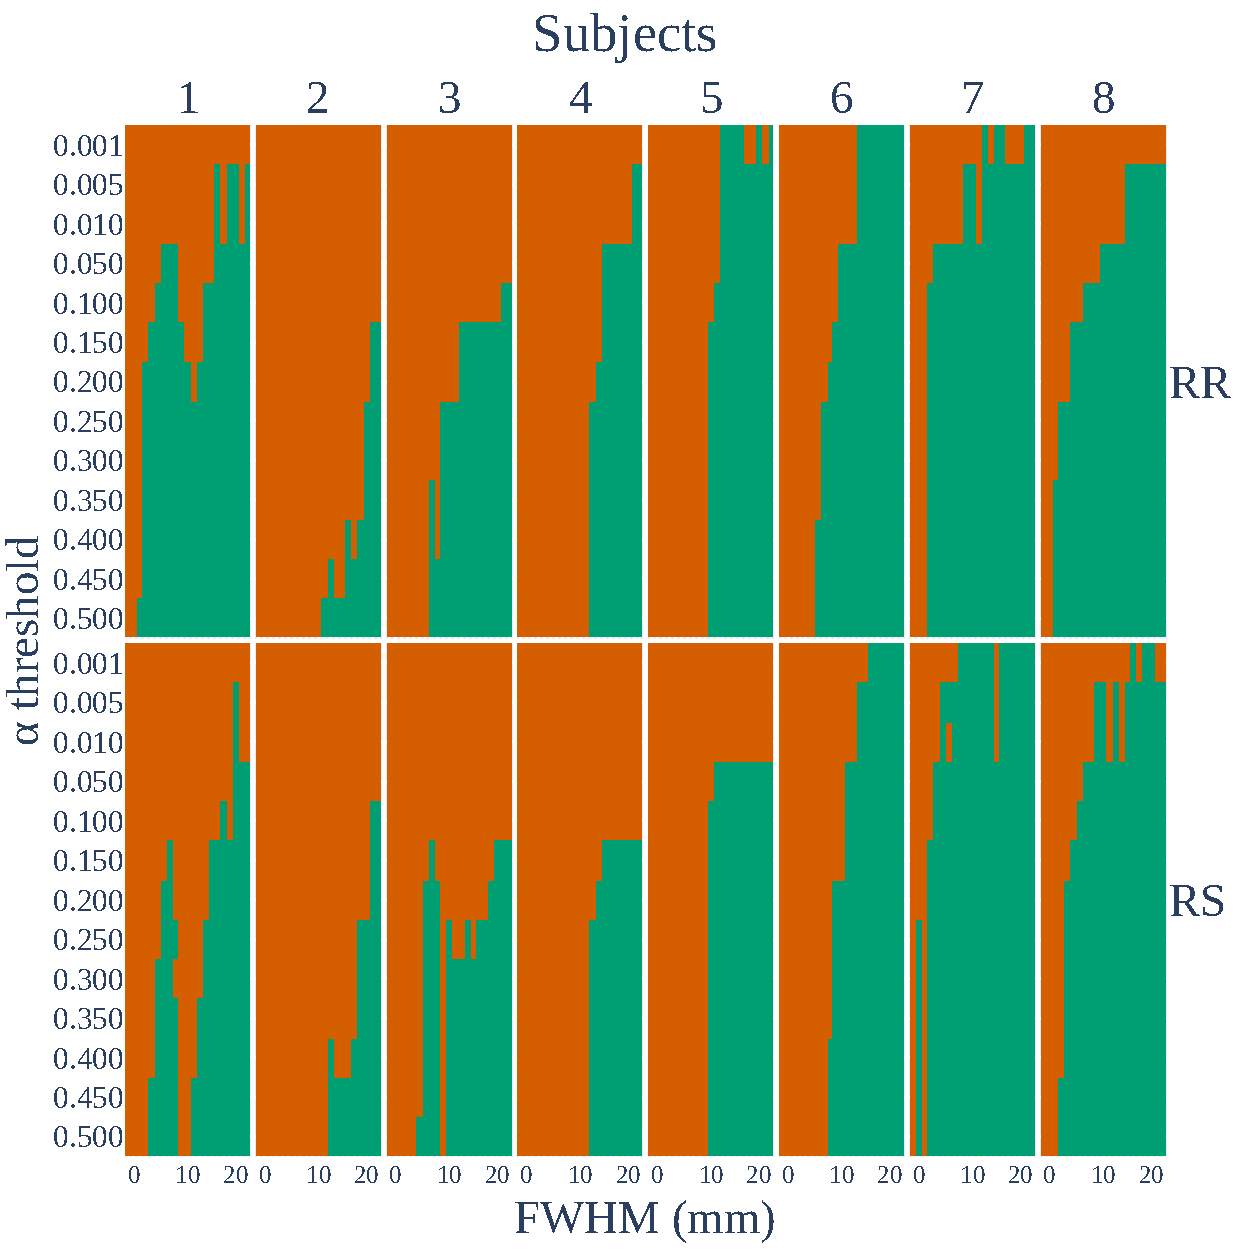
\includegraphics[width=\linewidth]{figures/loo_fwe_bonferroni.pdf}
    \caption{Leave-one-out evaluation of stability test for subjects 1 to 8.
        Red/green: rejected/accepted by a binomial one-tailed test with sample size $n=30$ and confidence level $1-\alpha_0=0.95$.}
    \label{fig:loo_bonferroni}
\end{figure}


\paragraph{IEEE check} We constructed the stability test from the $n$ perturbed results for each subject and applied it to the IEEE results (one per subject). The purpose of this check was twofold: (within subject) to verify that IEEE results passed the stability test built from the reference distribution of their corresponding subject and (between subjects) to verify that IEEE results failed the stability test built from the reference distribution of other subjects.

Within subject: for each subject there was an $\alpha$ and FWHM pair such that all the within-subject IEEE checks passed (Figure~\ref{fig:ieee-check}). In particular, the within-subject IEEE check passed with FWHM=15~mm for all subjects and $\alpha$ values for RR perturbations. For low FWHM sizes, the stability test rejected the IEEE sample of the reference subject, suggesting a lack of specificity in such cases.  

Between subjects: the stability tests successfully rejected all the IEEE samples coming from other subjects, for all combinations of $\alpha$ and FWHM values, and consistently for both RR and RS perturbations. Therefore the stability test is sufficiently sensitive to detect between-subject variability even with a high smoothing kernel size.

We conclude from this experiment that the stability test is sensitive enough to reject results obtained from different subjects using the reference application and accept results obtained from the same subject using the reference application executed with random perturbations.

\begin{figure}
    \centering
    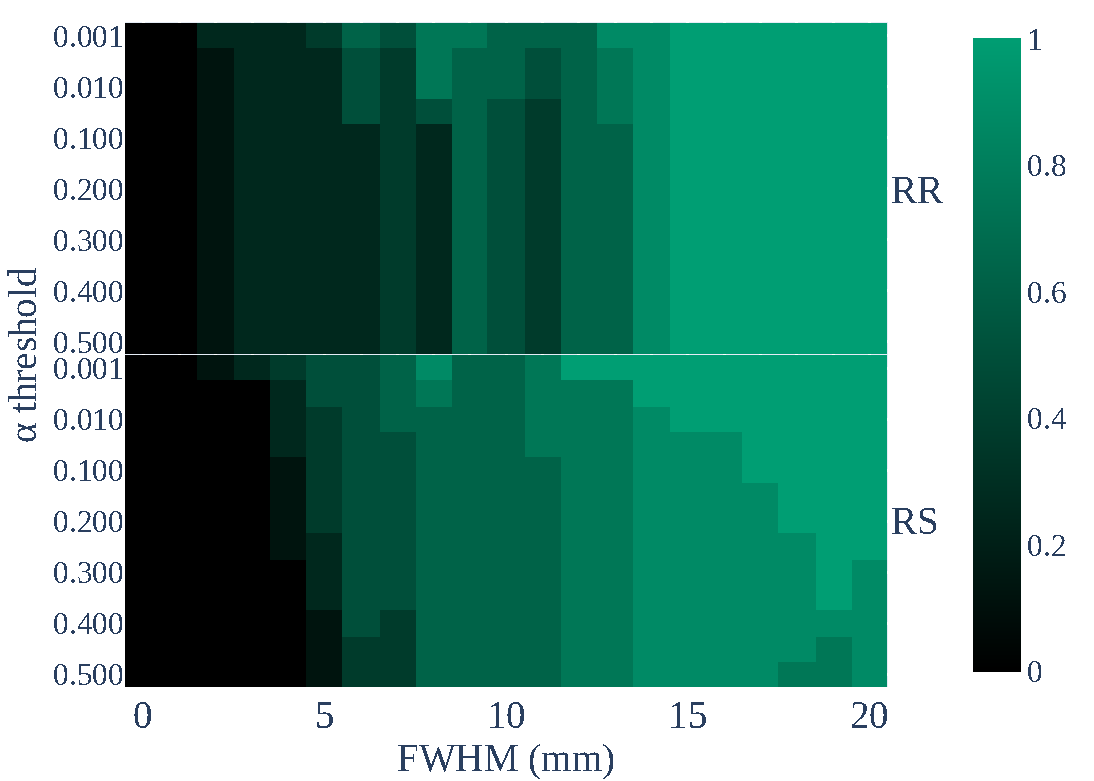
\includegraphics[width=\linewidth]{figures/inter-subject/inter_mct_fwe_bonferroni.pdf}
    \caption{Ratios of successful stability tests for the within-subject IEEE check. The between-subject IEEE check (not displayed in the figure) successfully rejected data computed from different subjects for all $\alpha$ and FWHM combinations, demonstrating excellent sensitivity.
    }
    \label{fig:ieee-check}
\end{figure}

\paragraph{Corrupted template check}

Multiple brain templates exist to spatially normalize subject data to a common space, and template selection substantially impacts the results~\cite{li2021moving}. Hence, errors in the template should lead to substantial differences in the results. The purpose of this check was to verify that results obtained from corrupted templates were correctly rejected by the stability test.
To do so, we generated corrupted versions of the MNI152NLin2009cAsym template used by \fmriprep where we incrementally zeroed the intensity of an increasing fraction of brain voxels selected uniformly. We then executed \fmriprep in IEEE mode (without random perturbations) for each resulting corrupted template and each subject.

The stability test correctly rejected results obtained with the corrupted template above a subject-dependent threshold of corrupted voxels (Figure~\ref{fig:template_bonferroni}). Smoothing had a measurable effect that did not manifest clearly across subjects. We conclude that the stability test is sensitive to changes in the brain template which are a common source of variability in neuroimaging.

% First, the sensitivity of the test to the "dead voxels" is not the same for each subject. On one hand, the test rejects subjects 3, 4, 5 and 6 for small percentages of noise ($\leq 1\%$) even for high FMWH levels. On the other hand, subjects 1, 2, 7 and 8 require a high percentage of noise (80\% for the highest level of smoothing) to be rejected by the test. This distinction between the two groups of subjects is correlated to the average number of significant bits (Figure~\ref{fig:significant-digits}), the first group being the one with the highest average number of significant bits. \TG{revise this parapgraph}
% This distinction is also clearly visible when we look at the uncertainty maps at FMWH=5mm (Figure~\ref{fig:uncertainty-maps-5mm}). This correlation may mean that the test is more permissive to a high percentage of "dead voxels" for subjects having the highest uncertainty (or lowest number of significant bits).

\begin{figure}
    \centering
    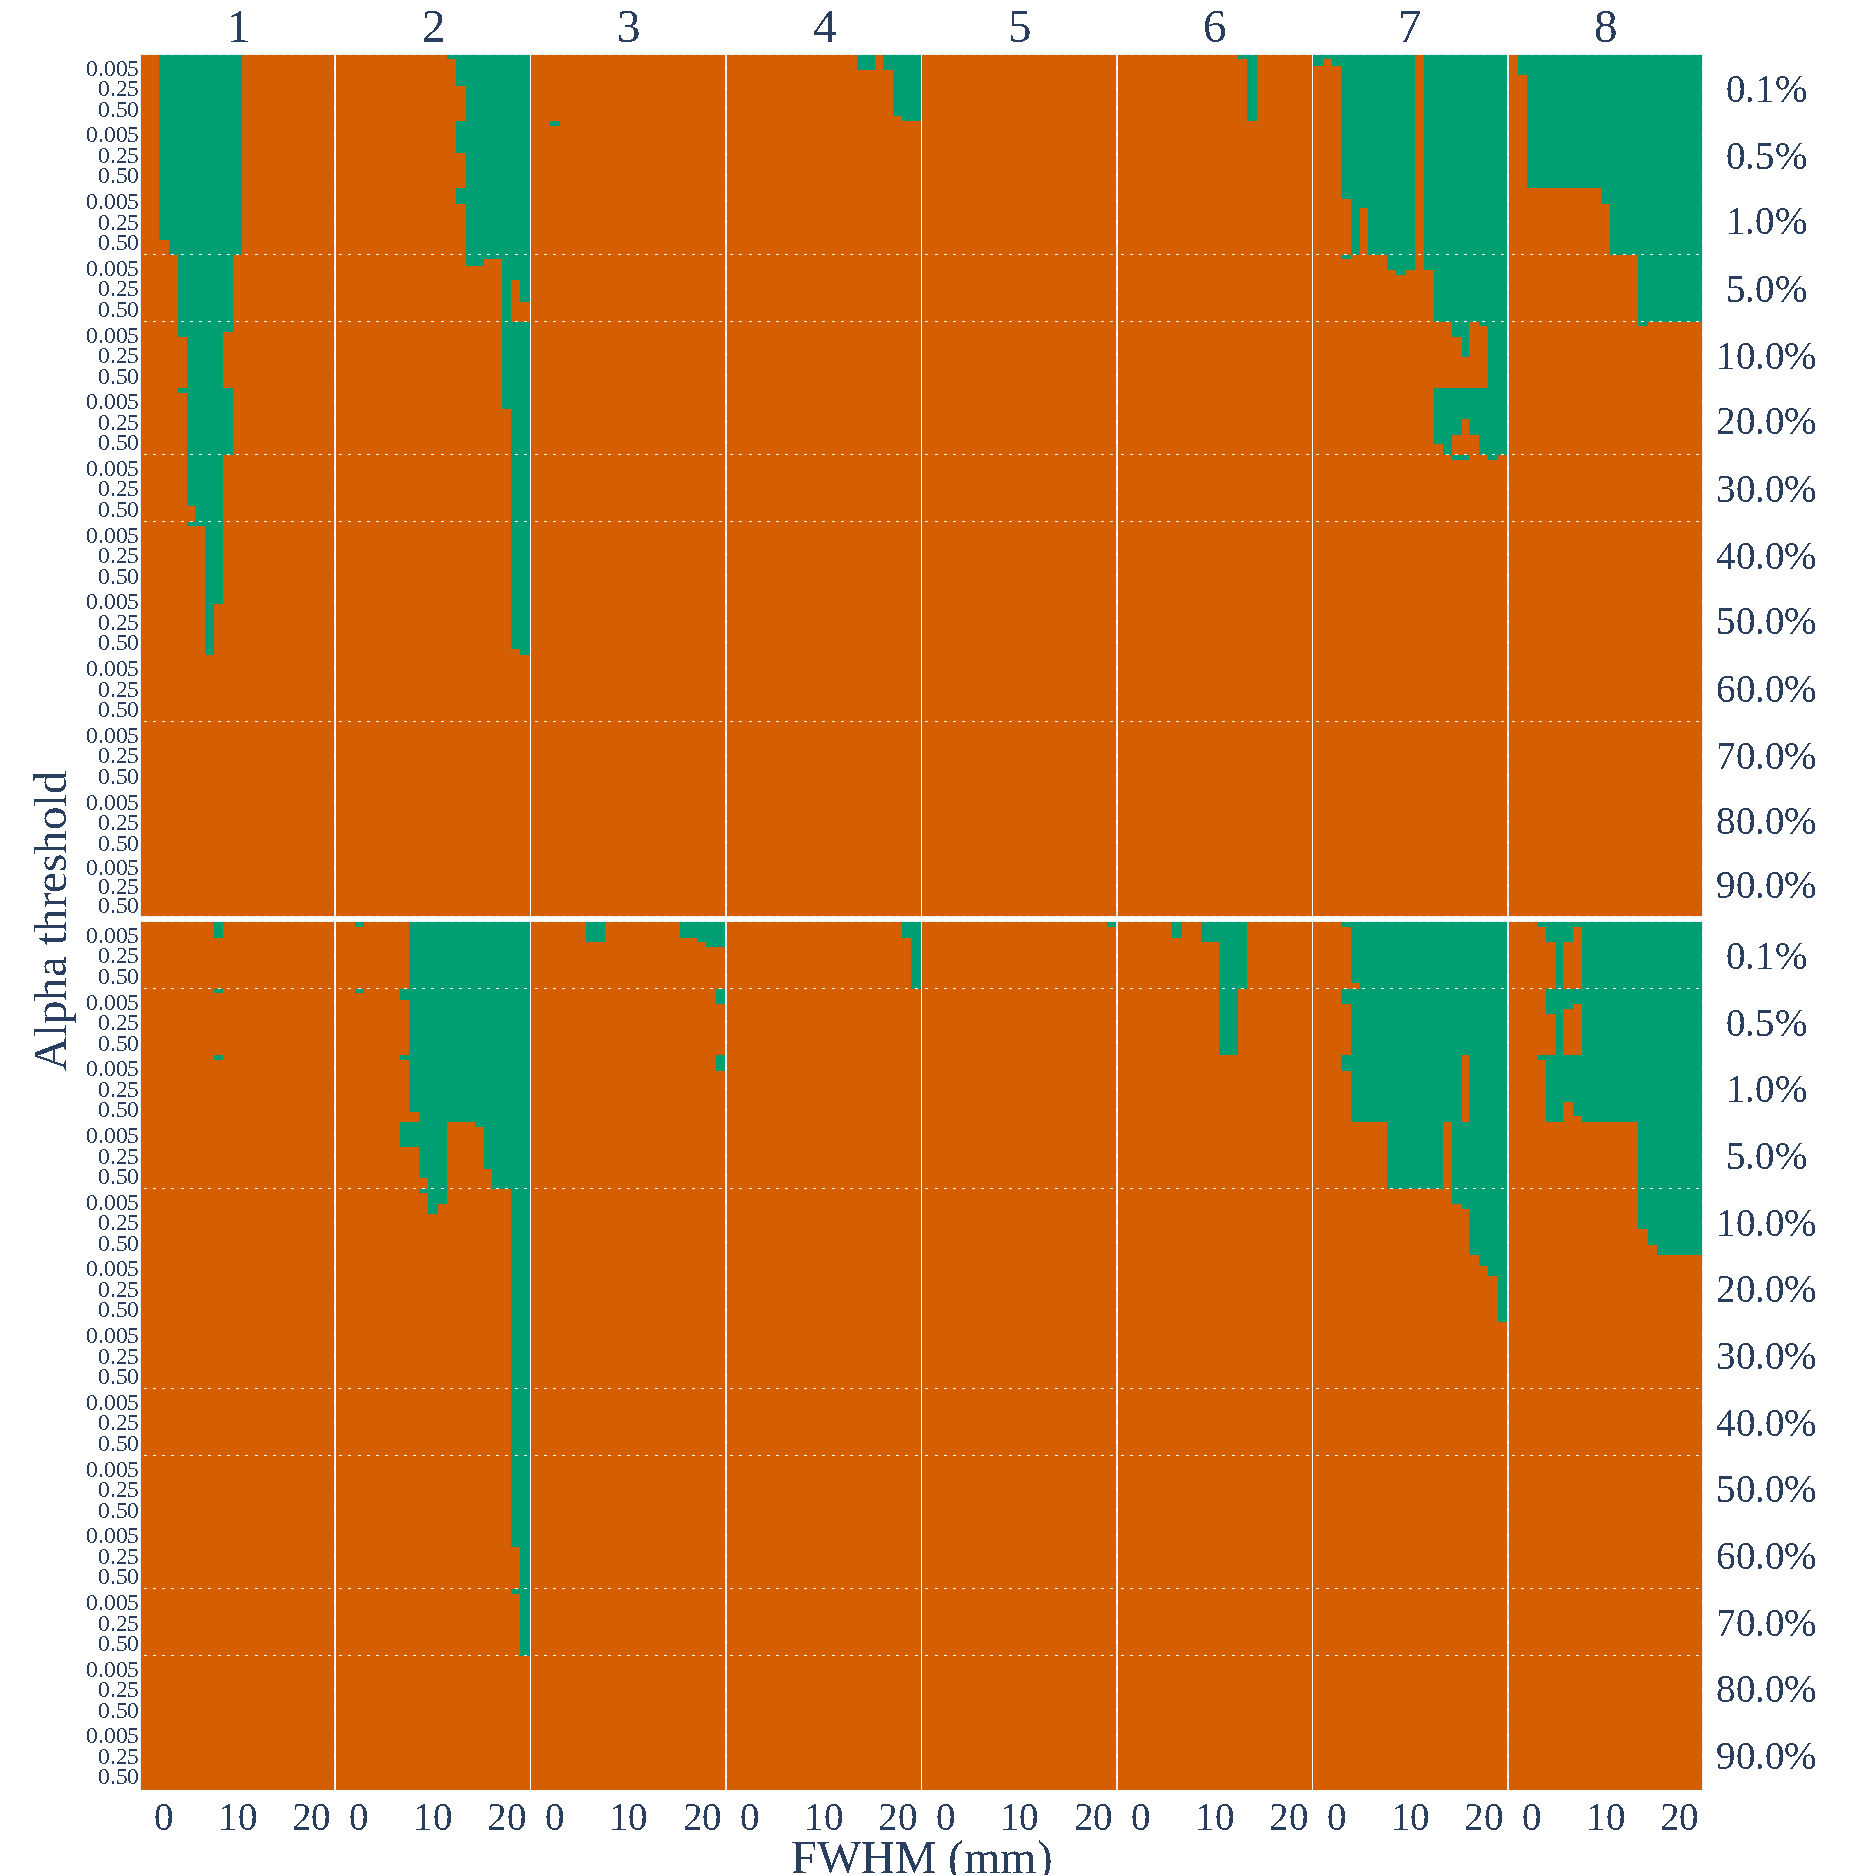
\includegraphics[width=\linewidth]{figures/template/template_fwe_bonferroni.pdf}
    \caption{Corrupted template check for RR (top) and RS (bottom) modes. \TG{RR, RS, and "fraction of corrupted voxels" should appear in the figure} The stability tests correctly rejected results produced with corrupted templates beyond a subject-dependent threshold of corrupted voxels.}
    \label{fig:template_bonferroni}
\end{figure}

% \subsection{The results stability test accepted CPU architecture variations}

%  The goal was to identify potential sources of variability in \fmriprep results more broadly. First, to test 
% variability across hardware architectures, we executed \fmriprep in IEEE mode in 6 different CPU architectures encountered in different computing clusters of the Digital Alliance of Canada \TG{right?}. The goal of this experiment was to explore whether hardware architecture has a measurable impact on \fmriprep results beyond numerical variability. \TG{Tristan to expand further depending on Yohan's current checks.}


% %  Figure~\ref{fig:arch_bonferroni} shows the results of the stability test for increasing $\alpha$ and FWHM values for RR and RS. We see that the architecture used has no impact on the stability test since results are identical across architecture for a subject and a perturbation mode given. For subject 1, we see that the variability of the stability test results is more important across perturbation modes.
% % In conclusion, the mode of perturbation used in constructing the test holds greater significance than the utilized architecture. This suggests that \fmriprep has low usage of specific hardware instructions, leading to a significant reduction in the variability generated across different architectures.

% \begin{figure}
%     \centering
%     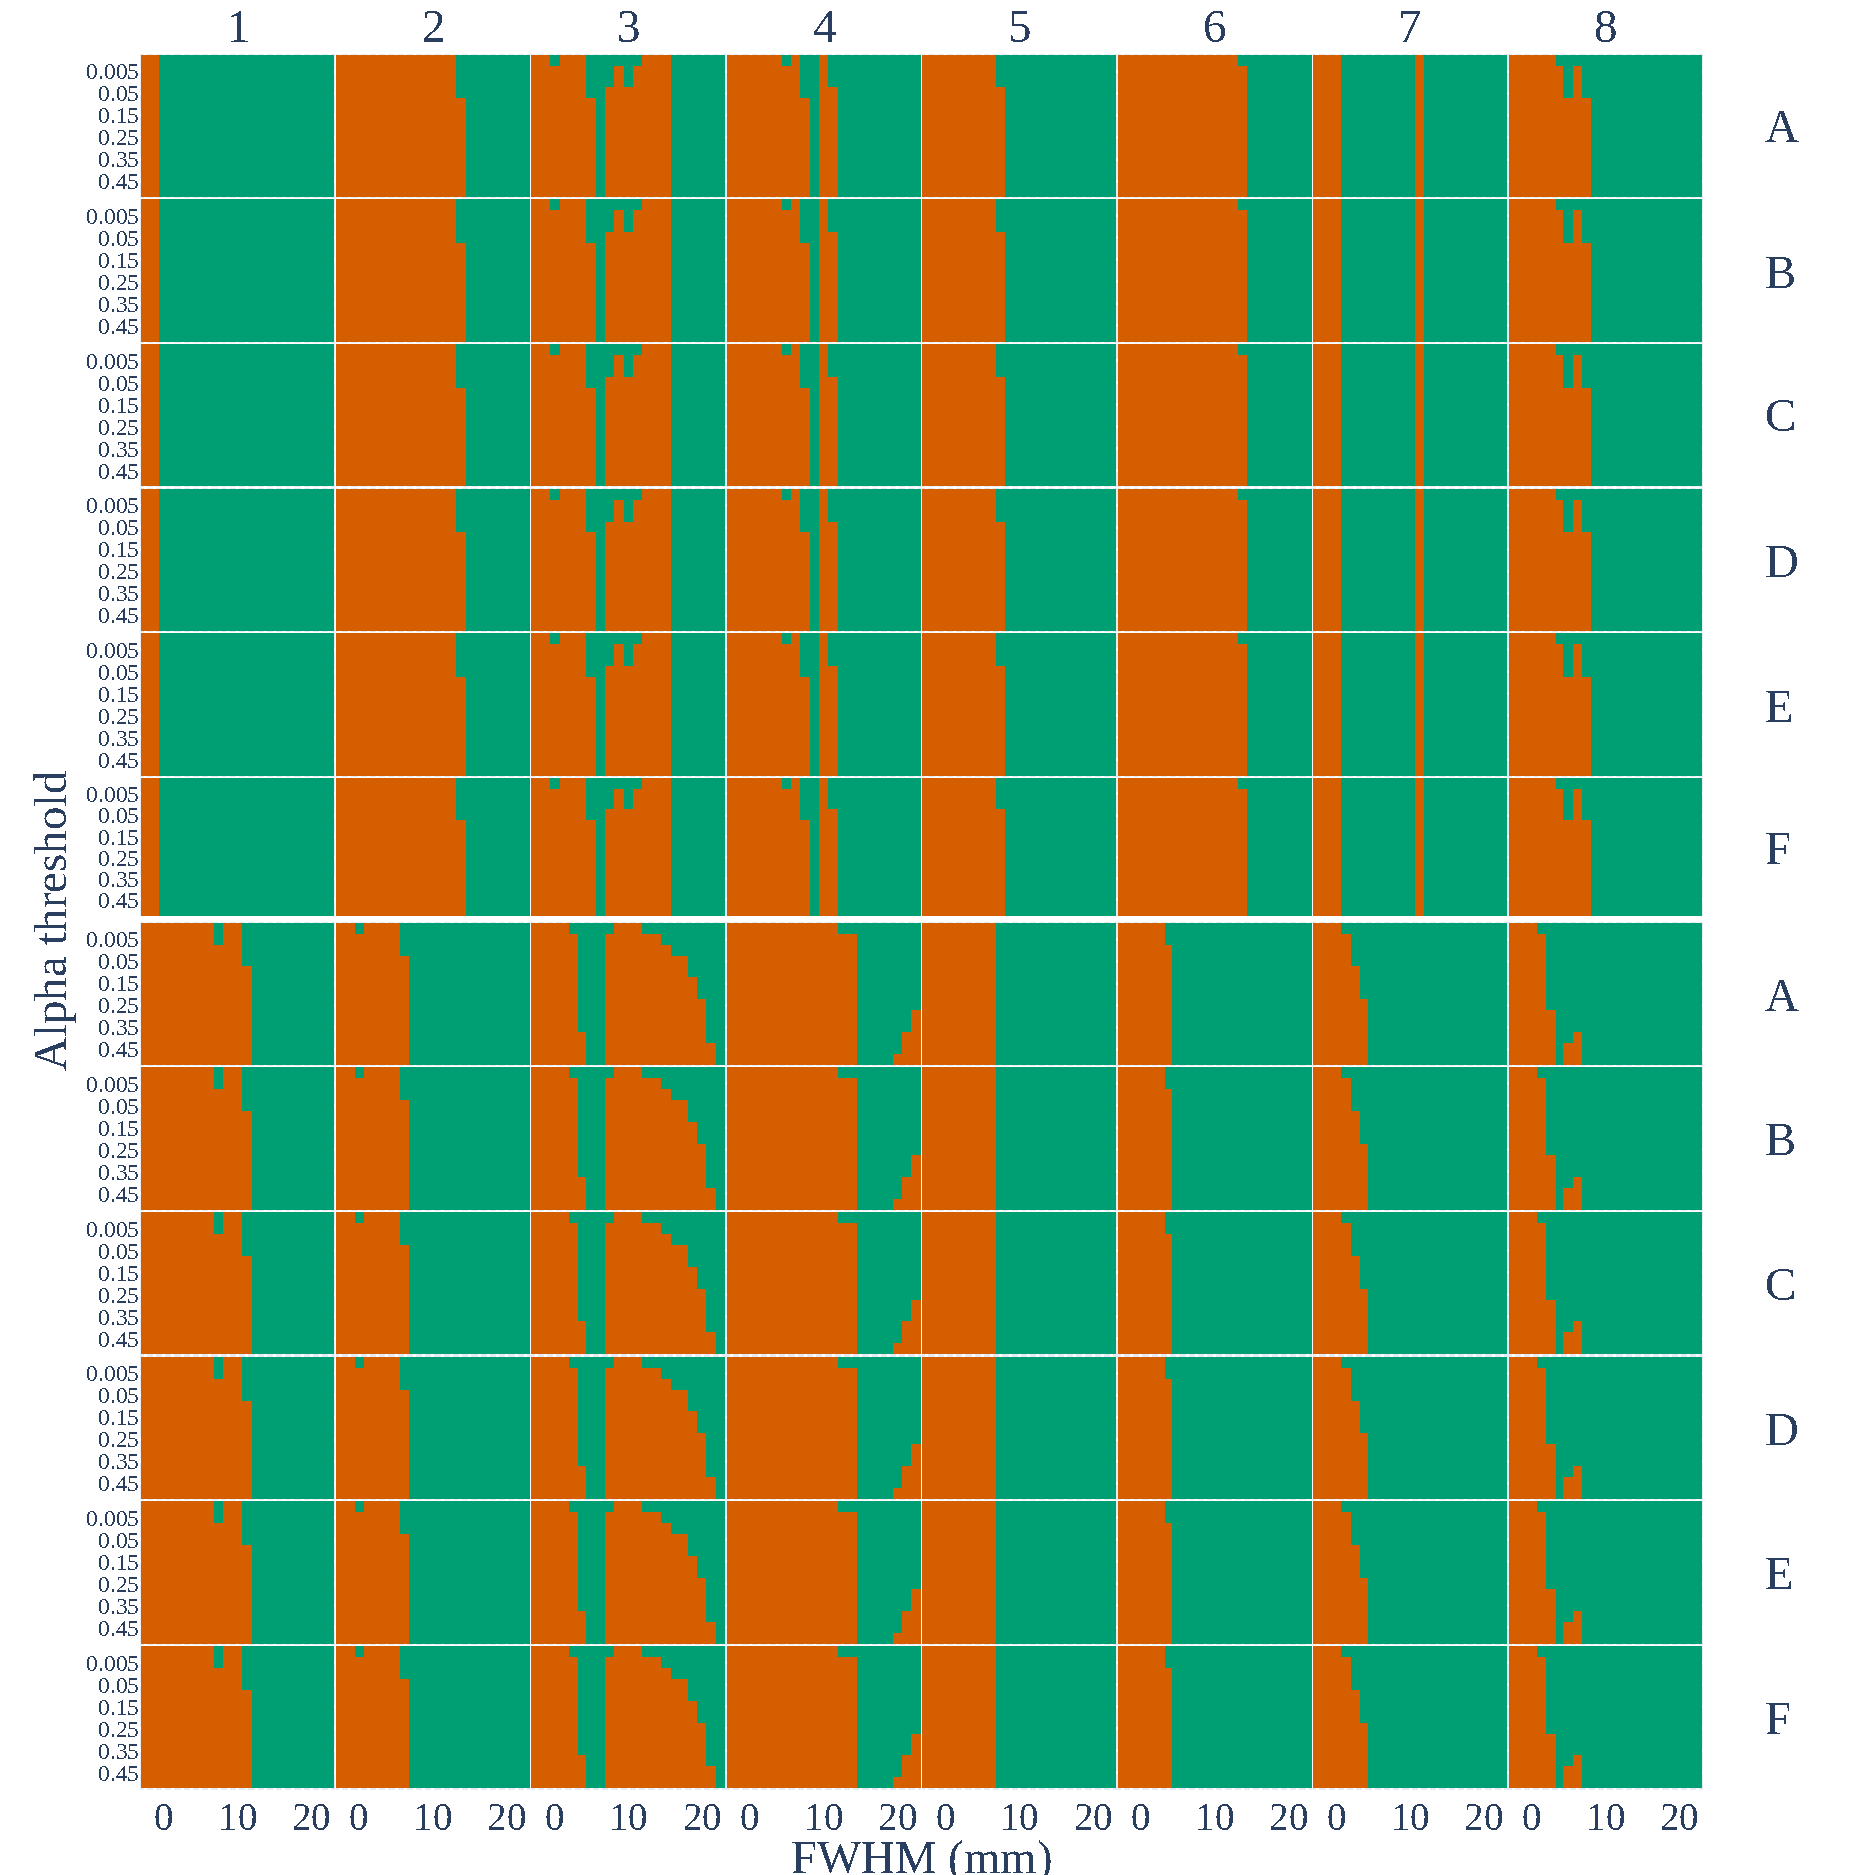
\includegraphics[width=\linewidth]{figures/arch/arch_fwe_bonferroni.pdf}
%     \caption{Stability test application to different CPU architectures for subjects 1 to 8. \TG{Mention RR and RS in the figure.} \TG{Mention which architecture was used to build the test} A: AMD Rome 7532; B: Intel E5-2683 v4 Broadwell; C: Intel Silver 4216 Cascade Lake; D: Intel Platinum 8160F Skylake; E: Intel Gold 5120 Skylake; F: Intel Gold 6238 Cascade Lake.}
%     \label{fig:arch_bonferroni}
% \end{figure}

\subsection{The results stability test detected subtle updates in \fmriprep image processing methods}

The previous sanity checks demonstrated a satisfying level of sensitivity and specificity of our stability test for simple scenarios. Subsequently, we applied it to our main motivating use case: the detection of results differences in \fmriprep LTS versions. We tested the results produced by different versions of \fmriprep, having built the results stability test for version \TG{x}. The goal of this experiment was to evaluate the ability of the stability test to detect significant software updates in \fmriprep. The stability test accepted results produced by versions 20.2.0 to 20.2.4 for all subjects (Figure~\ref{fig:version_bonferroni}). However, the test rejected results produced by versions 20.2.5 and onwards, suggesting a substantial change in the analysis methods from version 20.2.5. Investigations with the \fmriprep developers revealed that the interpolation scheme involved in the resampling of the segmented brain maps from MGZ format into NiFTI was changed in version {20.2.5} from trilinear interpolation to nearest neighbor (see PR \href{https://github.com/nipreps/smriprep/pull/268}{\url{github.com/nipreps/smriprep/pull/268}}). The ability of our results stability test to detect such subtle changes in the analysis supports its relevance fin the release process of long-term support data analysis software.

\begin{figure}
    \centering
    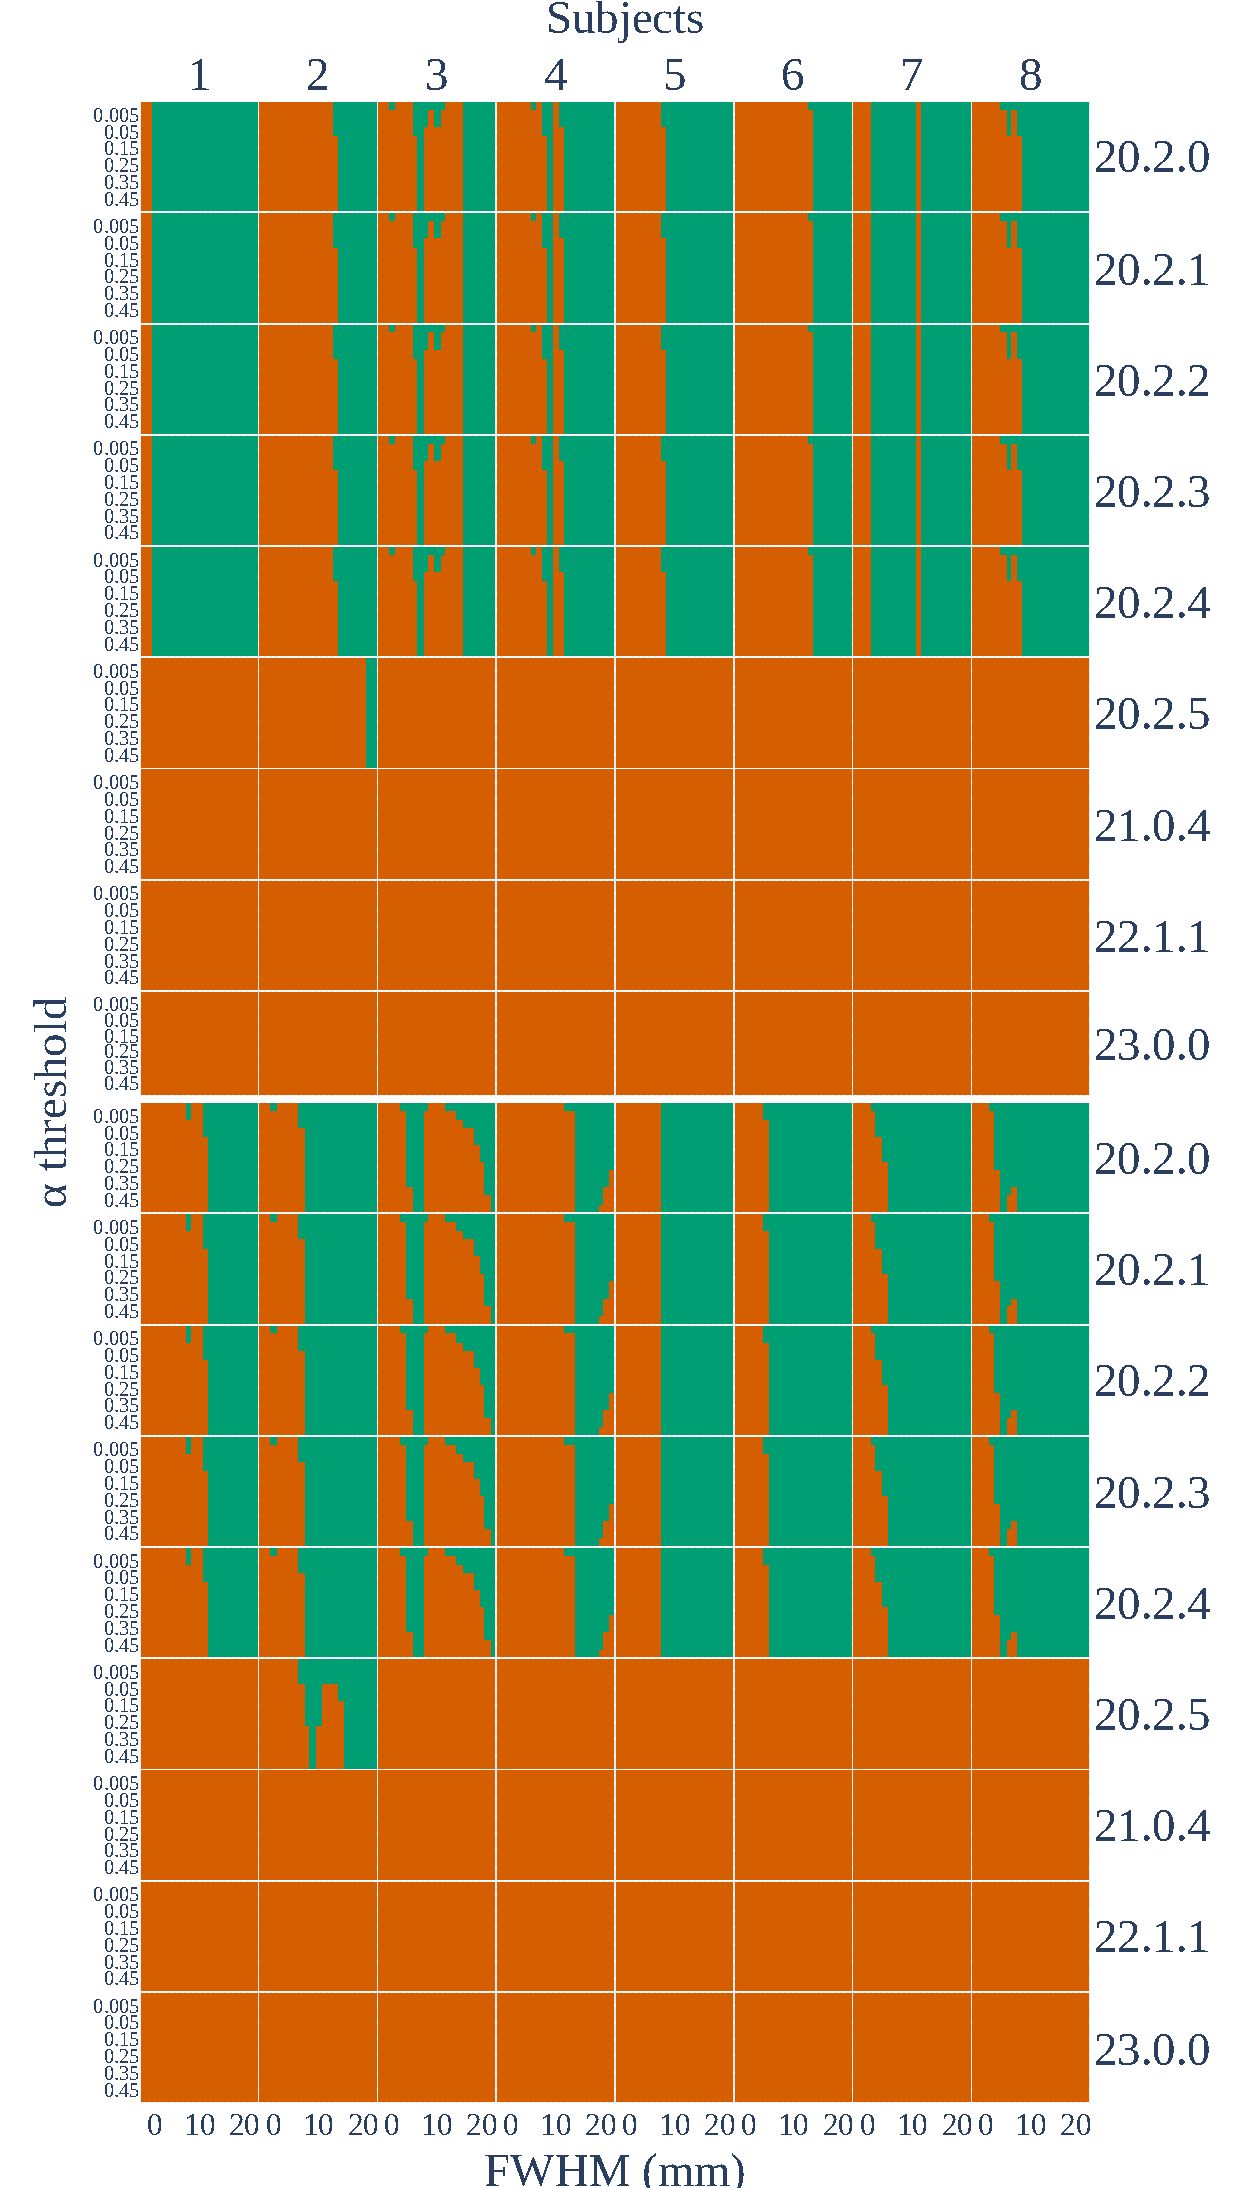
\includegraphics[width=\linewidth]{figures/fmriprep-versions/versions_fwe_bonferroni.pdf}
    \caption{Stability test application to different \fmriprep versions.}
    \label{fig:version_bonferroni}
\end{figure}


\section{Discussion}

% summary of results

We have proposed the first approach to build stability tests for numerical analysis in the absence of an exact solution, a reference solution and even an acceptable bound of variation around the computed solution. We have applied this approach to \fmriprep, one of the largest processing pipelines in neuroimaging and we have demonstrated that our approach can detect variabilities coming from different \fmriprep versions.

The numerical stability of the results varied across subjects in our study. Subjects were chosen to reflect diverse acquisition qualities, resolutions, ages, and genders. Although our analysis did not precisely determine which factors specifically influenced the stability test, we observed that certain smoothing sizes were more appropriate than others, indicating an optimal smoothing bandwidth.

Fuzzy-libmath provides an independent method to evaluate the numerical quality of neuroimaging pipelines since it generates variability comparable to random-seed. The smoothing size tended to affect the performance of the stability test, as it rendered the distribution of voxels more normal. However, voxel-wise analysis prevented the prediction of excessively large non-local variations. Incorporating neighborhood information could improve learning, such as using more general deep learning methods like VoxelMorph~\cite{balakrishnan2019voxelmorph}.

The assumption of normality simplifies calculations. The issue with non-parametric methods is that they require large sample sizes ($>100$) to achieve an acceptable confidence level ($>0.95$). However, the acquisition cost for \fmriprep and neuroimaging pipelines in general is prohibitively high in terms of time and storage space. Working on other outputs, such as regions of interest with the produced segmentations, could reduce the volume of elements to be processed and enable more complex analyses in computations.

The solutions obtained for the smoothing kernel size may not be anatomically satisfactory for neuroimaging researchers (FWHM $\geq 15$) in terms of anatomical accuracy, but they are valid from a software engineering perspective, as they allow for the detection of significant changes between different versions of \fmriprep. Although our methods may not be currently applicable for neuroimaging research stricto sensu, they serve as a stability test for identifying noticeable differences between computed outputs.

The Bonferroni correction, although conservative, fails to capture observations from reference distributions, as demonstrated by LOO (Figure~\ref{fig:loo_bonferroni}) and IEEE (Figure~\ref{fig:ieee-check}) checks. This could be attributed to two factors. Firstly, voxels in neuroimaging data are not spatially independent, and secondly, perturbed samples used in the analysis are not independent due to the optimization problems involved in pre-processing, such as spatial normalization and bias field correction. These optimization problems do not have analytical solutions and require numerical methods for addressing them. However, due to the inherent complexity of these problems (\cite{clarenz2006computational}), even small perturbations in the input data can result in substantially different but equally valid computed solutions. As a consequence, minimal variations in calculations introduced by Fuzzy-libmath can lead to significantly different geometric solutions, resulting in regions of high instability within anatomical brain images, particularly at white/grey matter borders (Figure~\ref{fig:uncertainty-maps}). And so when working voxel-wise, the obtained brain geometries can differ significantly at the voxel level, transitioning from intensity levels characteristic of gray matter to white matter, and vice versa. Furthermore, subsampling the solution space of optimization problems may lead to the omission of possible white matter regions where only gray matter was observed, and vice versa.

Nevertheless, our method is sufficiently precise to detect inter-subject variability, even at higher levels of smoothing. The numerical perturbations introduced by Fuzzy-libmath only affect a small portion of the calculations performed in \fmriprep. Although it reproduces the measured variability by varying the random seed, it does not stimulate calculations performed elsewhere in advancing neuroimaging. Extending the test to other application domains where the libmath has little effect on stability~\cite{pepe2022numerical} will require perturbing other computation libraries.

Finally, our method is designed for data that are independent collections of numerical values and does not take into account particular geometries. For example, we treat all spatial axes of the T1 images as equivalent without privileging any particular axis. Furthermore, we consider the absolute value of elements, such as voxel intensity in our case, rather than the relative differences between them. In future work, we plan to extend our test to other types of data, such as those used in functional neuroimaging. In functional neuroimaging, researchers analyze time series of neural activations and are primarily interested in activation potential rather than the absolute magnitude of voxel intensity. Additionally, the treatment of the time axis is different from that of the spatial axes. We will therefore have to take into account time dependencies.

\section{Conclusion}

We have proposed a novel approach for building stability tests in numerical analysis, even in the absence of an exact solution, a reference solution, or an acceptable bound of variation around the computed solution. We applied this approach to \fmriprep, one of the largest processing pipelines in neuroimaging, and demonstrated its ability to detect variabilities across different \fmriprep versions.

From a software engineering perspective, our stability test applies to a carefully selected database of test subjects, as we were able to identify valid configurations $\alpha$ and FWHM for which the test passed our sanity checks. The identified configurations varied across subjects, depending on the quality of the acquisition data, indicating that our test is robust to heterogeneously quality data.

From a neuroimaging perspective, our analyses revealed significant discrepancies in numerical quality results after preprocessing, with an average of 2 to 10 bits out of 12 bits available. The quality of results varied considerably with the acquisition quality and the chosen random seed. Additionally, spatial smoothing had a notable impact on improving result quality, with improvements of 2 to 10 bits observed for some subjects.

Furthermore, we demonstrated that the Fuzzy-libmath perturbations type yielded comparable numerical quality results to those obtained with random seeds, highlighting the ability of the Monte Carlo arithmetic approach to accurately simulate numerical instabilities.
% However, it should be noted that some specific random seeds resulted in considerably higher variability, as shown by the results from subject 7 in RR+RS modes (Figure~\ref{fig:uncertainty-maps}).

Our results showed that our test is more sensitive (i.e., has a higher ability to correctly detect true positives) than specific (i.e., has a higher ability to correctly detect true negatives). Specifically, our method exhibited lower specificity for low FWHM values, likely due to the voxel-wise analysis that does not account for neighborhood effects and poor sampling space. This limitation arises from the computational cost of statistical analyses and the acquisition cost of perturbed results. However, our test demonstrated high sensitivity, as we were able to correctly reject target images from different subjects or with low to moderate levels of noise in the brain template, depending on the applied FWHM.

In conclusion, our proposed stability test represents a novel and effective method for detecting code changes that result in substantial numerical variabilities within results represented as numerical structured grids. By providing a method that relies on a numerical values sample and does not require ad-hoc assumptions specific to a particular numerical scheme, our approach offers a flexible and widely applicable solution for stability testing in numerical analysis.
Through our demonstrations on a large neuroimaging pipeline, such as \fmriprep, for the preprocessing step, we have shown the effectiveness of our approach under assumptions of independence and normality.

In future research, we plan to extend our methodology to other data types and investigate its applicability under different statistical hypotheses. This work has the potential to contribute to the development of robust stability tests for numerical analysis in diverse scientific domains beyond neuroimaging, further enhancing the reliability and reproducibility of computational results.

\section{Acknowledgments}

Computations were made on the Narval supercomputer from \'Ecole de Technologie
Sup\'erieure (ETS, Montr\'eal), managed by Calcul Québec and the Digital Research Alliance of Canada. The
operation of this supercomputer is funded by the Canada Foundation for
Innovation (CFI), Ministère de l’Économie, des Sciences et de l’Innovation du
Québec (MESI) and le Fonds de recherche du Québec – Nature et technologies
(FRQ-NT).

\bibliographystyle{IEEEtran}
\bibliography{main}


\appendix

\section{Numerical variability results for different smoothing kernel sizes}
\label{appendix:numerical_uncertainty}

% \begin{landscape}
%     \begin{figure}
%         \vspace*{-2cm}
%         \centering
%         \uncertaintyMap{0}{1}{ds000256}{sub-CTS201}[true] \\
%         \uncertaintyMap{0}{2}{ds000256}{sub-CTS210} \\
%         \uncertaintyMap{0}{3}{ds001600}{sub-1} \\
%         \uncertaintyMap{0}{4}{ds001748}{sub-adult15} \\
%         \uncertaintyMap{0}{5}{ds001748}{sub-adult16} \\
%         \uncertaintyMap{0}{6}{ds001771}{sub-36} \\
%         \uncertaintyMap{0}{7}{ds002338}{sub-xp201} \\
%         \uncertaintyMap{0}{8}{ds002338}{sub-xp207} \\
%         \includegraphics*[width=.7\linewidth]{figures/colorbar_sigbit.pdf}
%         \caption{Uncertainty measured for subjects 1 to 8 (from top to bottom) across n=30 perturbed samples, with FWHM=0mm. }
%         \label{fig:uncertainty-maps-0mm}
%     \end{figure}
% \end{landscape}

% \begin{landscape}
%     \begin{figure}
%         \vspace*{-2cm}
%         \centering
%         \uncertaintyMap{5}{1}{ds000256}{sub-CTS201}[true] \\
%         \uncertaintyMap{5}{2}{ds000256}{sub-CTS210} \\
%         \uncertaintyMap{5}{3}{ds001600}{sub-1} \\
%         \uncertaintyMap{5}{4}{ds001748}{sub-adult15} \\
%         \uncertaintyMap{5}{5}{ds001748}{sub-adult16} \\
%         \uncertaintyMap{5}{6}{ds001771}{sub-36} \\
%         \uncertaintyMap{5}{7}{ds002338}{sub-xp201} \\
%         \uncertaintyMap{5}{8}{ds002338}{sub-xp207} \\
%         \includegraphics*[width=.7\linewidth]{figures/colorbar_sigbit.pdf}
%         \caption{Uncertainty measured for subjects 1 to 8 (from top to bottom) across n=30 perturbed samples, with FWHM=5mm. }
%         \label{fig:uncertainty-maps-5mm}
%     \end{figure}
% \end{landscape}

% \begin{landscape}
%     \begin{figure}
%         \vspace*{-2cm}
%         \centering
%         \uncertaintyMap{10}{1}{ds000256}{sub-CTS201}[true] \\
%         \uncertaintyMap{10}{2}{ds000256}{sub-CTS210} \\
%         \uncertaintyMap{10}{3}{ds001600}{sub-1} \\
%         \uncertaintyMap{10}{4}{ds001748}{sub-adult15} \\
%         \uncertaintyMap{10}{5}{ds001748}{sub-adult16} \\
%         \uncertaintyMap{10}{6}{ds001771}{sub-36} \\
%         \uncertaintyMap{10}{7}{ds002338}{sub-xp201} \\
%         \uncertaintyMap{10}{8}{ds002338}{sub-xp207} \\
%         \includegraphics*[width=.7\linewidth]{figures/colorbar_sigbit.pdf}
%         \caption{Uncertainty measured for subjects 1 to 8 (from top to bottom) across n=30 perturbed samples, with FWHM=10mm. }
%         \label{fig:uncertainty-maps-10mm}
%     \end{figure}
% \end{landscape}

% \begin{landscape}
%     \begin{figure}
%         \vspace*{-2cm}
%         \centering
%         \uncertaintyMap{20}{1}{ds000256}{sub-CTS201}[true] \\
%         \uncertaintyMap{20}{2}{ds000256}{sub-CTS210} \\
%         \uncertaintyMap{20}{3}{ds001600}{sub-1} \\
%         \uncertaintyMap{20}{4}{ds001748}{sub-adult15} \\
%         \uncertaintyMap{20}{5}{ds001748}{sub-adult16} \\
%         \uncertaintyMap{20}{6}{ds001771}{sub-36} \\
%         \uncertaintyMap{20}{7}{ds002338}{sub-xp201} \\
%         \uncertaintyMap{20}{8}{ds002338}{sub-xp207} \\
%         \includegraphics*[width=.7\linewidth]{figures/colorbar_sigbit.pdf}
%         \caption{Uncertainty measured for subjects 1 to 8 (from top to bottom) across n=30 perturbed samples, with FWHM=20mm. }
%         \label{fig:uncertainty-maps-20mm}
%     \end{figure}
% \end{landscape}


\begin{landscape}
    \begin{figure}
        \vspace*{-2cm}
        \centering
        \uncertaintyMapDiscrete{0}{1}{ds000256}{sub-CTS201}[true] \\
        \uncertaintyMapDiscrete{0}{2}{ds000256}{sub-CTS210} \\
        \uncertaintyMapDiscrete{0}{3}{ds001600}{sub-1} \\
        \uncertaintyMapDiscrete{0}{4}{ds001748}{sub-adult15} \\
        \uncertaintyMapDiscrete{0}{5}{ds001748}{sub-adult16} \\
        \uncertaintyMapDiscrete{0}{6}{ds001771}{sub-36} \\
        \uncertaintyMapDiscrete{0}{7}{ds002338}{sub-xp201} \\
        \uncertaintyMapDiscrete{0}{8}{ds002338}{sub-xp207} \\
        \includegraphics*[width=.7\linewidth]{figures/colorbar_sigbit_discrete.pdf}
        \caption{Numerical variability measured for subjects 1 to 8 (from top to bottom) across n=30 perturbed samples, with FWHM=0mm. }
        \label{fig:uncertainty-maps-0mm-disc}
    \end{figure}
\end{landscape}

\begin{landscape}
    \begin{figure}
        \vspace*{-2cm}
        \centering
        \uncertaintyMapDiscrete{5}{1}{ds000256}{sub-CTS201}[true] \\
        \uncertaintyMapDiscrete{5}{2}{ds000256}{sub-CTS210} \\
        \uncertaintyMapDiscrete{5}{3}{ds001600}{sub-1} \\
        \uncertaintyMapDiscrete{5}{4}{ds001748}{sub-adult15} \\
        \uncertaintyMapDiscrete{5}{5}{ds001748}{sub-adult16} \\
        \uncertaintyMapDiscrete{5}{6}{ds001771}{sub-36} \\
        \uncertaintyMapDiscrete{5}{7}{ds002338}{sub-xp201} \\
        \uncertaintyMapDiscrete{5}{8}{ds002338}{sub-xp207} \\
        \includegraphics*[width=.7\linewidth]{figures/colorbar_sigbit_discrete.pdf}
        \caption{Numerical variability measured for subjects 1 to 8 (from top to bottom) across n=30 perturbed samples, with FWHM=5mm. }
        \label{fig:uncertainty-maps-5mm-disc}
    \end{figure}
\end{landscape}

\begin{landscape}
    \begin{figure}
        \vspace*{-2cm}
        \centering
        \uncertaintyMapDiscrete{10}{1}{ds000256}{sub-CTS201}[true] \\
        \uncertaintyMapDiscrete{10}{2}{ds000256}{sub-CTS210} \\
        \uncertaintyMapDiscrete{10}{3}{ds001600}{sub-1} \\
        \uncertaintyMapDiscrete{10}{4}{ds001748}{sub-adult15} \\
        \uncertaintyMapDiscrete{10}{5}{ds001748}{sub-adult16} \\
        \uncertaintyMapDiscrete{10}{6}{ds001771}{sub-36} \\
        \uncertaintyMapDiscrete{10}{7}{ds002338}{sub-xp201} \\
        \uncertaintyMapDiscrete{10}{8}{ds002338}{sub-xp207} \\
        \includegraphics*[width=.7\linewidth]{figures/colorbar_sigbit_discrete.pdf}
        \caption{Numerical variability measured for subjects 1 to 8 (from top to bottom) across n=30 perturbed samples, with FWHM=10mm. }
        \label{fig:uncertainty-maps-10mm-disc}
    \end{figure}
\end{landscape}

\begin{landscape}
    \begin{figure}
        \vspace*{-2cm}
        \centering
        \uncertaintyMapDiscrete{20}{1}{ds000256}{sub-CTS201}[true] \\
        \uncertaintyMapDiscrete{20}{2}{ds000256}{sub-CTS210} \\
        \uncertaintyMapDiscrete{20}{3}{ds001600}{sub-1} \\
        \uncertaintyMapDiscrete{20}{4}{ds001748}{sub-adult15} \\
        \uncertaintyMapDiscrete{20}{5}{ds001748}{sub-adult16} \\
        \uncertaintyMapDiscrete{20}{6}{ds001771}{sub-36} \\
        \uncertaintyMapDiscrete{20}{7}{ds002338}{sub-xp201} \\
        \uncertaintyMapDiscrete{20}{8}{ds002338}{sub-xp207} \\
        \includegraphics*[width=.7\linewidth]{figures/colorbar_sigbit_discrete.pdf}
        \caption{Numerical variability measured for subjects 1 to 8 (from top to bottom) across n=30 perturbed samples, with FWHM=20mm. }
        \label{fig:uncertainty-maps-20mm-disc}
    \end{figure}
\end{landscape}


% \section{Colors Palette}
% Fail: \texttt{\#D55E00}
% Pass: \texttt{\#009E73}

% \section{Results for uncorrected tests}
% \label{appendix:multiple-comparison-tests}

% In the absence of multiple comparison corrections, we expect
% by construction to incorrectly reject each $H_{0,i}$ with probability $\alpha$ a.k.a
% the per-comparison error rate (PCER). To account for the PCER, we measure the
% fraction of positive z-tests $V_P$ among the $v$ voxels in the image and the
% tested \fmriprep result is considered part of the reference distribution iif:
% \begin{equation}
%     V_{P} \leq \alpha.
%     \label{eqn:pce}
% \end{equation}

% For each of the $n$ repetitions,
% we measured $V_P$, the fraction of
% positive z-tests among the $v$ voxels as well as $\mathds{1}_n$, the number of repetitions
% that passed the test with Bonferroni correction.

% For the uncorrected tests (Equation~\ref{eqn:pce}), we expect $\overline{V_P}$ to have
% the following upper bound:
% \[
%     \overline{V_P} \leq
%     \alpha  + t_{29,0.05} \frac{\tilde{\sigma}_{V_P}}{\sqrt{30}}
% \]
% with
% $t_{k,\gamma}$ the $(1-\gamma)$quantile of the Student distribution with $k$ degrees of freedom,
% and $\overline{V_P}$ and $\tilde{\sigma}_{V_P}$ the mean and standard-deviation estimated from
% $n$ $V_P$ measures.
% This confidence interval is obtained from a two-tailed one-sample
% t-test with $n-1$ degrees of freedom at a level of significance $\alpha_0=0.05$:
% \[
%     \mathbb{P}
%     \left(
%     -t_{n-1,\alpha_0/2}
%     <
%     \dfrac{\overline{V_p} - \alpha}{\tilde{\sigma}_{V_P} / \sqrt{n}}
%     <
%     t_{n-1,\alpha_0/2}
%     \right)
%     = 1 - \alpha_0
% \]

% fraction of positive
% z-tests $V_P$ among the $v$ voxels should be close to the nomimal value $\alpha$
% on average. To assess the validity of our LOO test, we test that the average
% of the $n$ $V_P$ fractions measured belongs to a confidence interval
% around the nomimal value $\alpha$. To do so, we use  resulting in the
% following confidence interval for $V_P$:

% obtained from:

% \begin{figure}
%     \centering
%     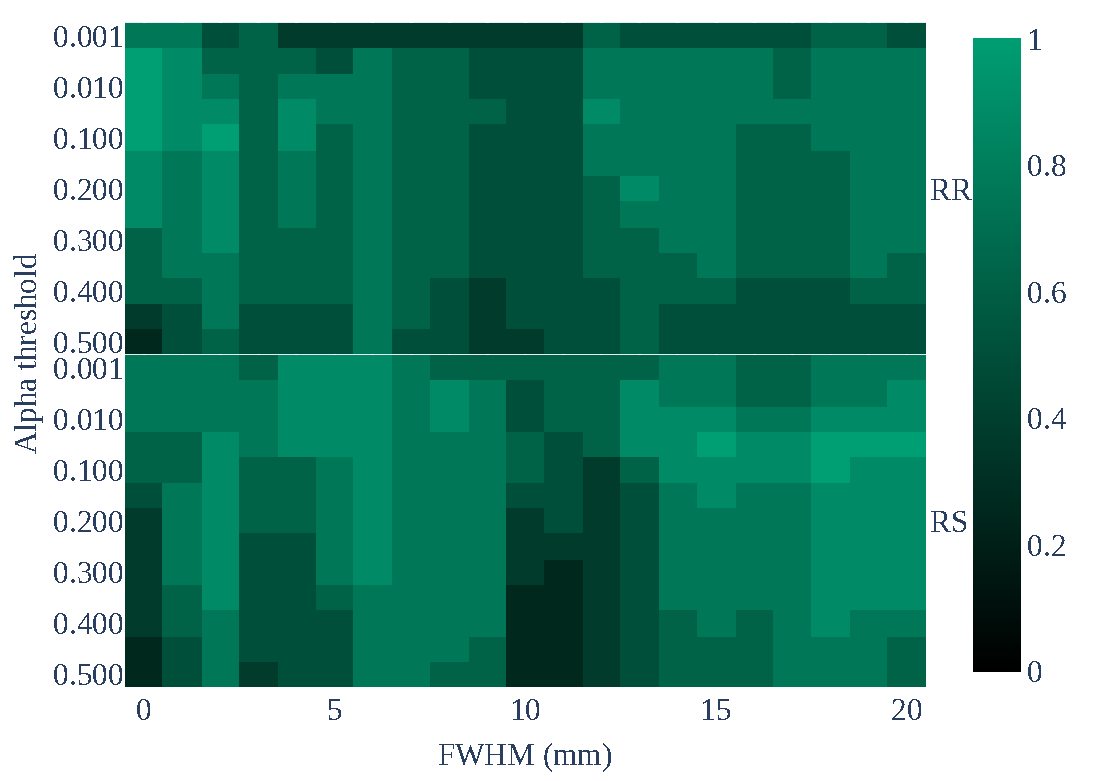
\includegraphics[width=\linewidth]{figures/inter-subject/inter_pce.pdf}
%     \caption{Inter-subject check for the uncorrected test for RR (top) and RS (bottom) modes. We expect that the tests would pass along the diagonals and be rejected otherwise.
%         Out of a total of 17,472 individual assessments, we reported 791 failures in the RR mode, representing a failure rate of 0.05\%, and 685 failures in the RS mode, corresponding to a failure rate of 0.04\%. These data corroborate our test's capacity to discern inter-subject variability.
%     }
%     \label{fig:ieee-check-pce}
% \end{figure}


% \begin{figure}
%     \centering
%     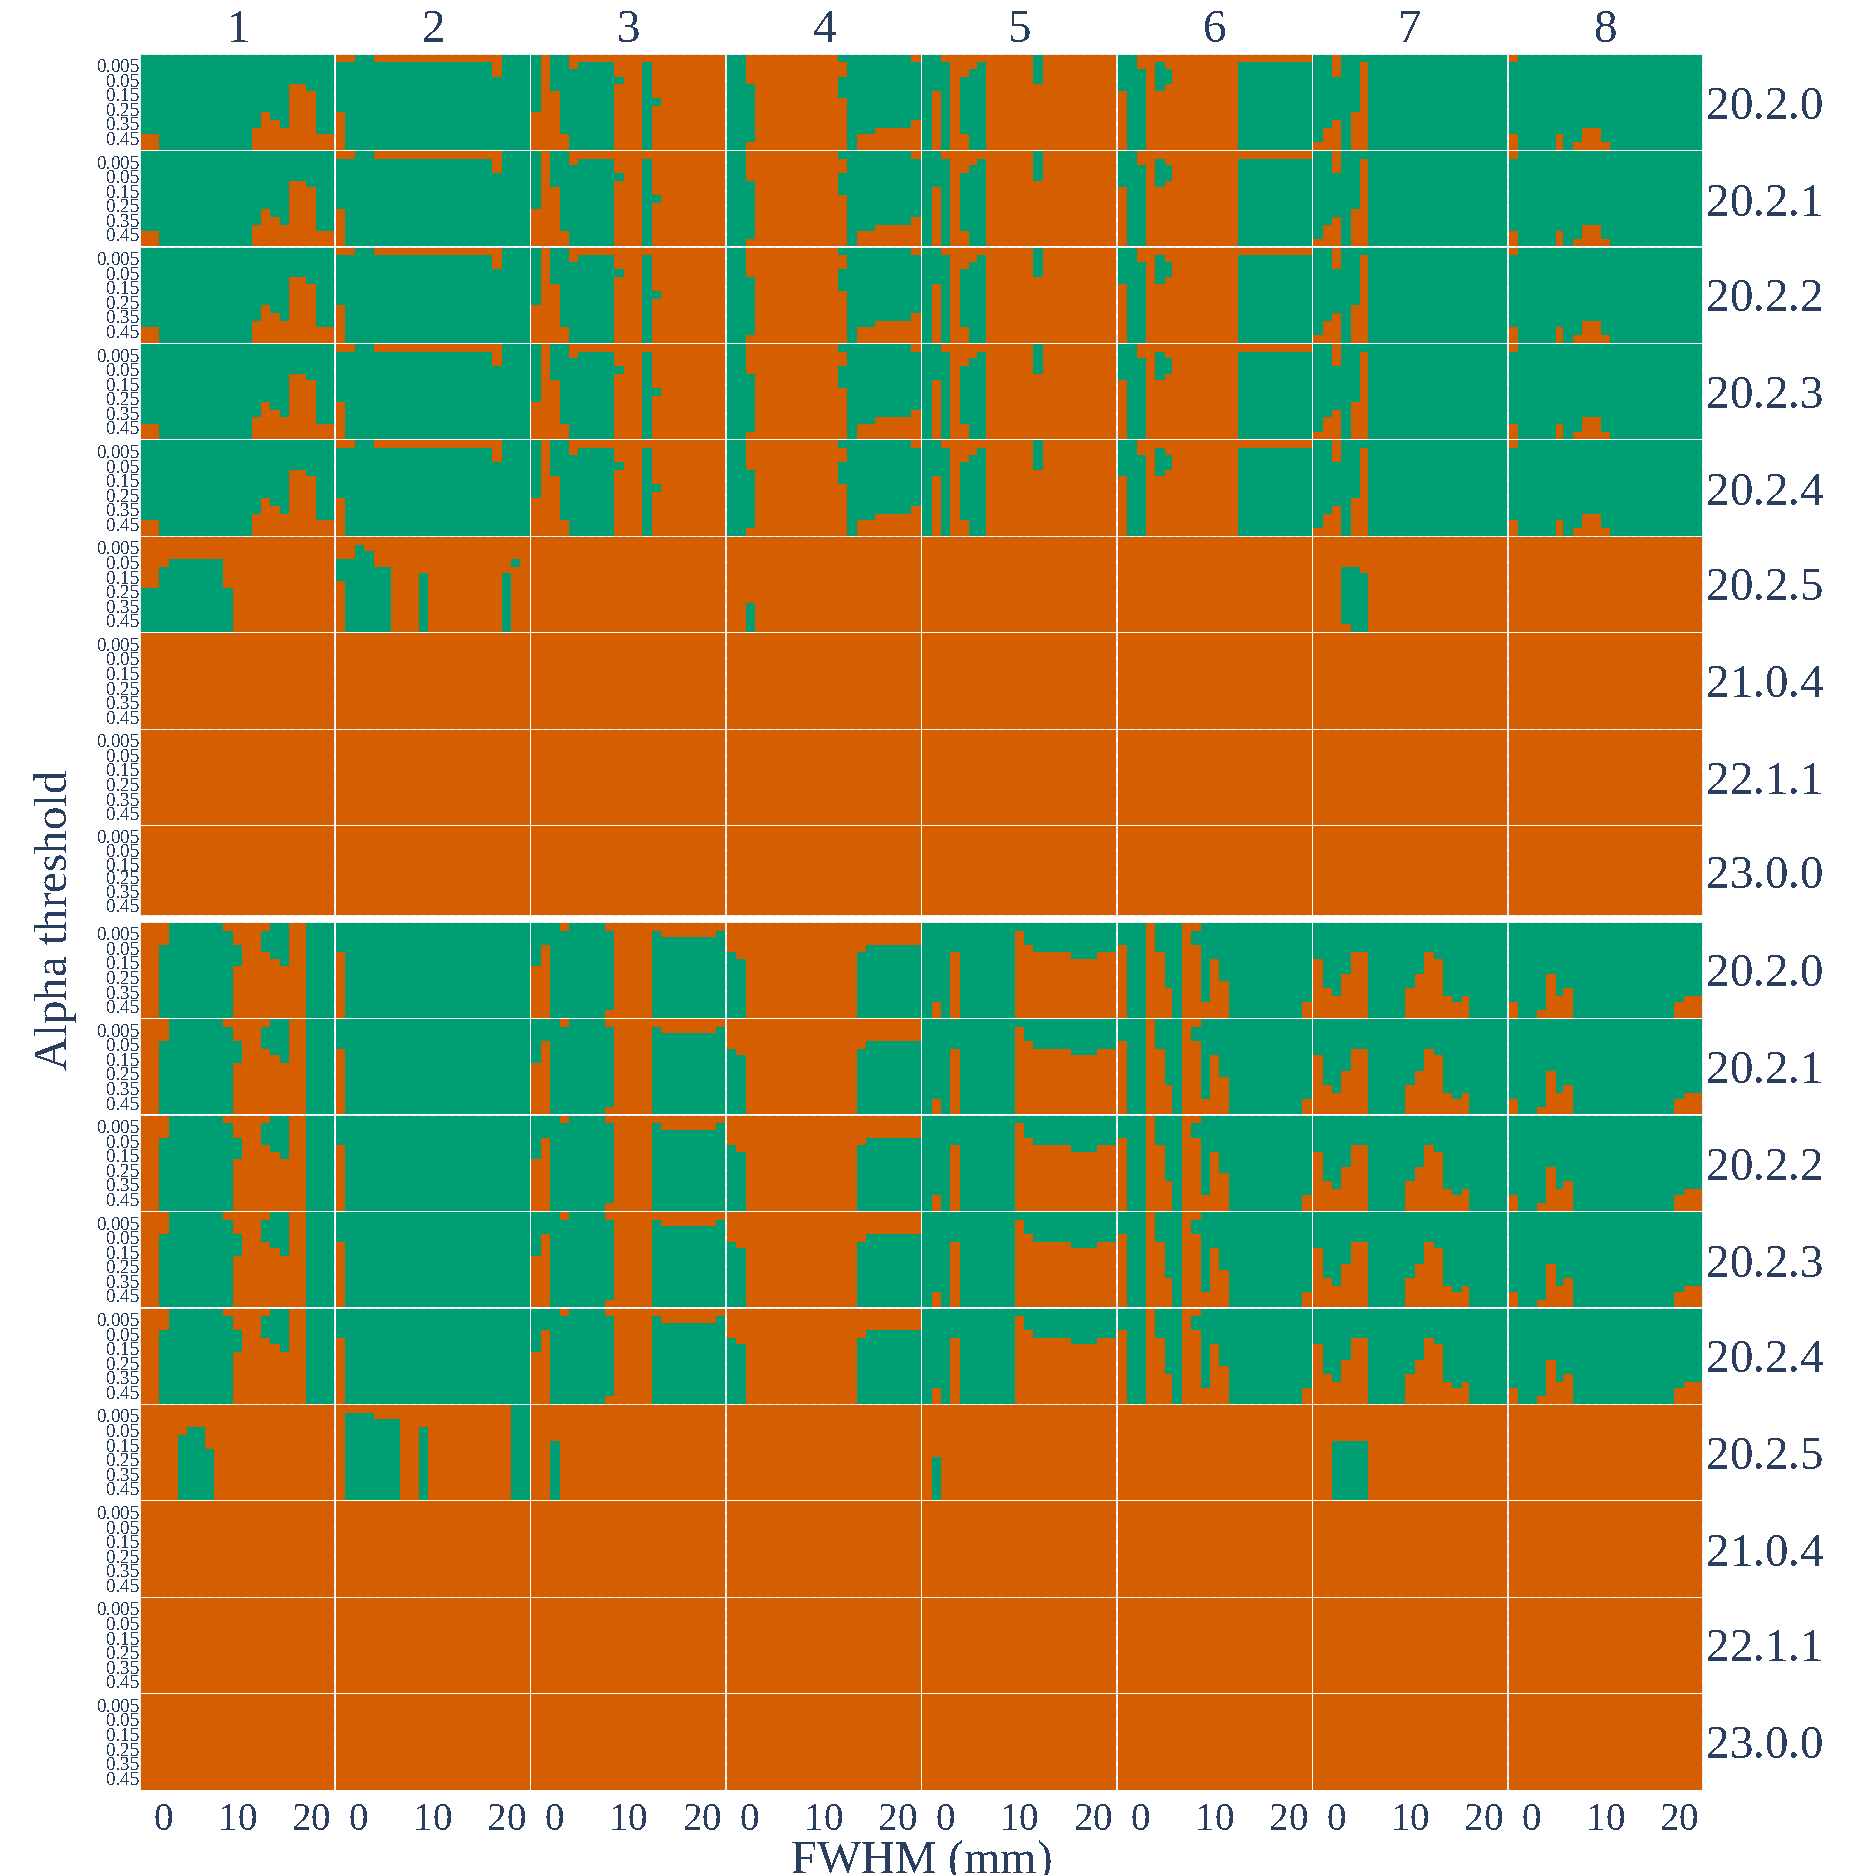
\includegraphics[width=\linewidth]{figures/fmriprep-versions/versions_pce.pdf}
%     \caption{Uncorrected test applications on different \fmriprep versions.}
%     \label{fig:versions_pce}
% \end{figure}

% \begin{figure}
%     \centering
%     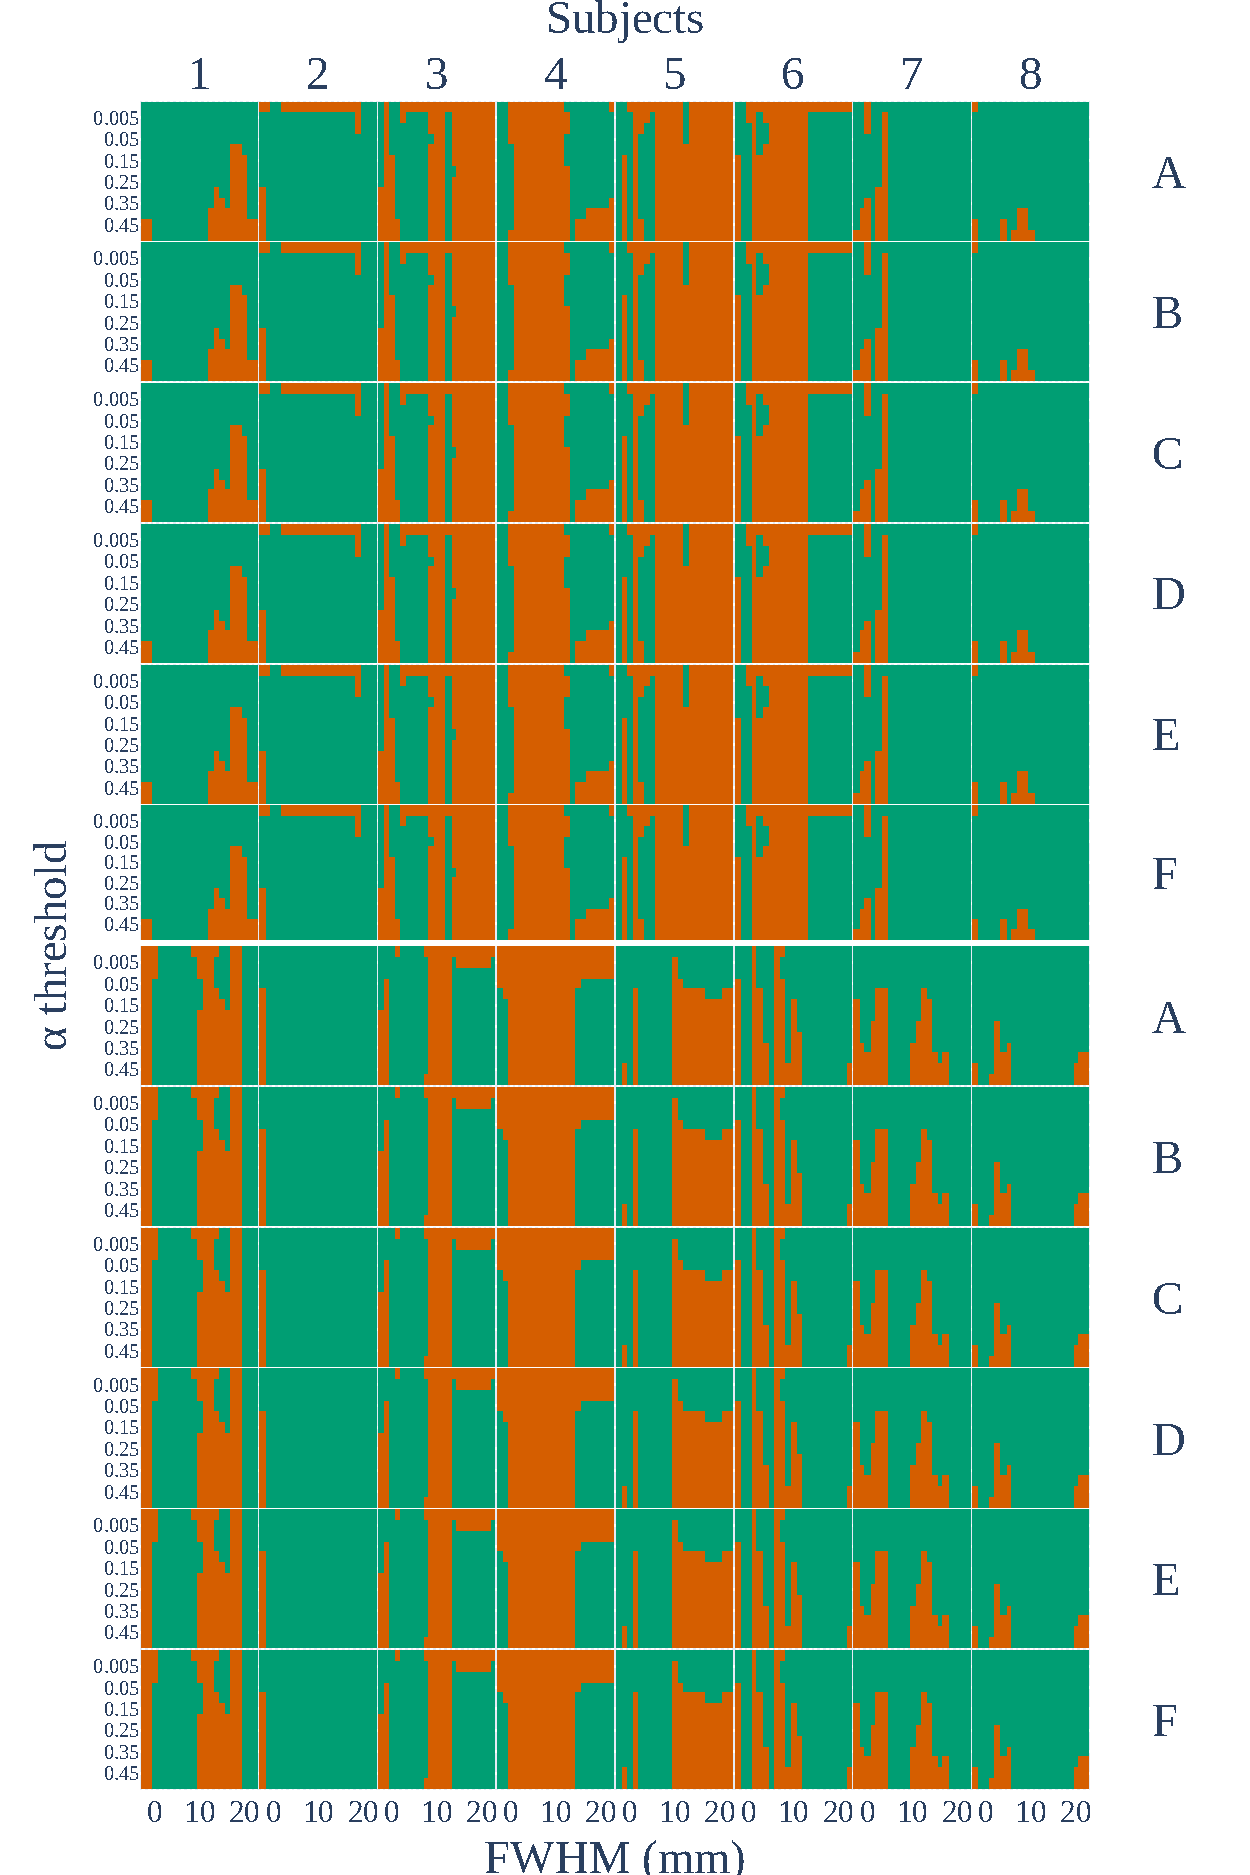
\includegraphics[width=\linewidth]{figures/arch/arch_pce.pdf}
%     \caption{Uncorrected test applications on CPU architectures.}
%     \label{fig:arch_pce}
% \end{figure}


% \section{Uncertainty maps for others FWHM}

% \begin{figure}
%     \centering
%     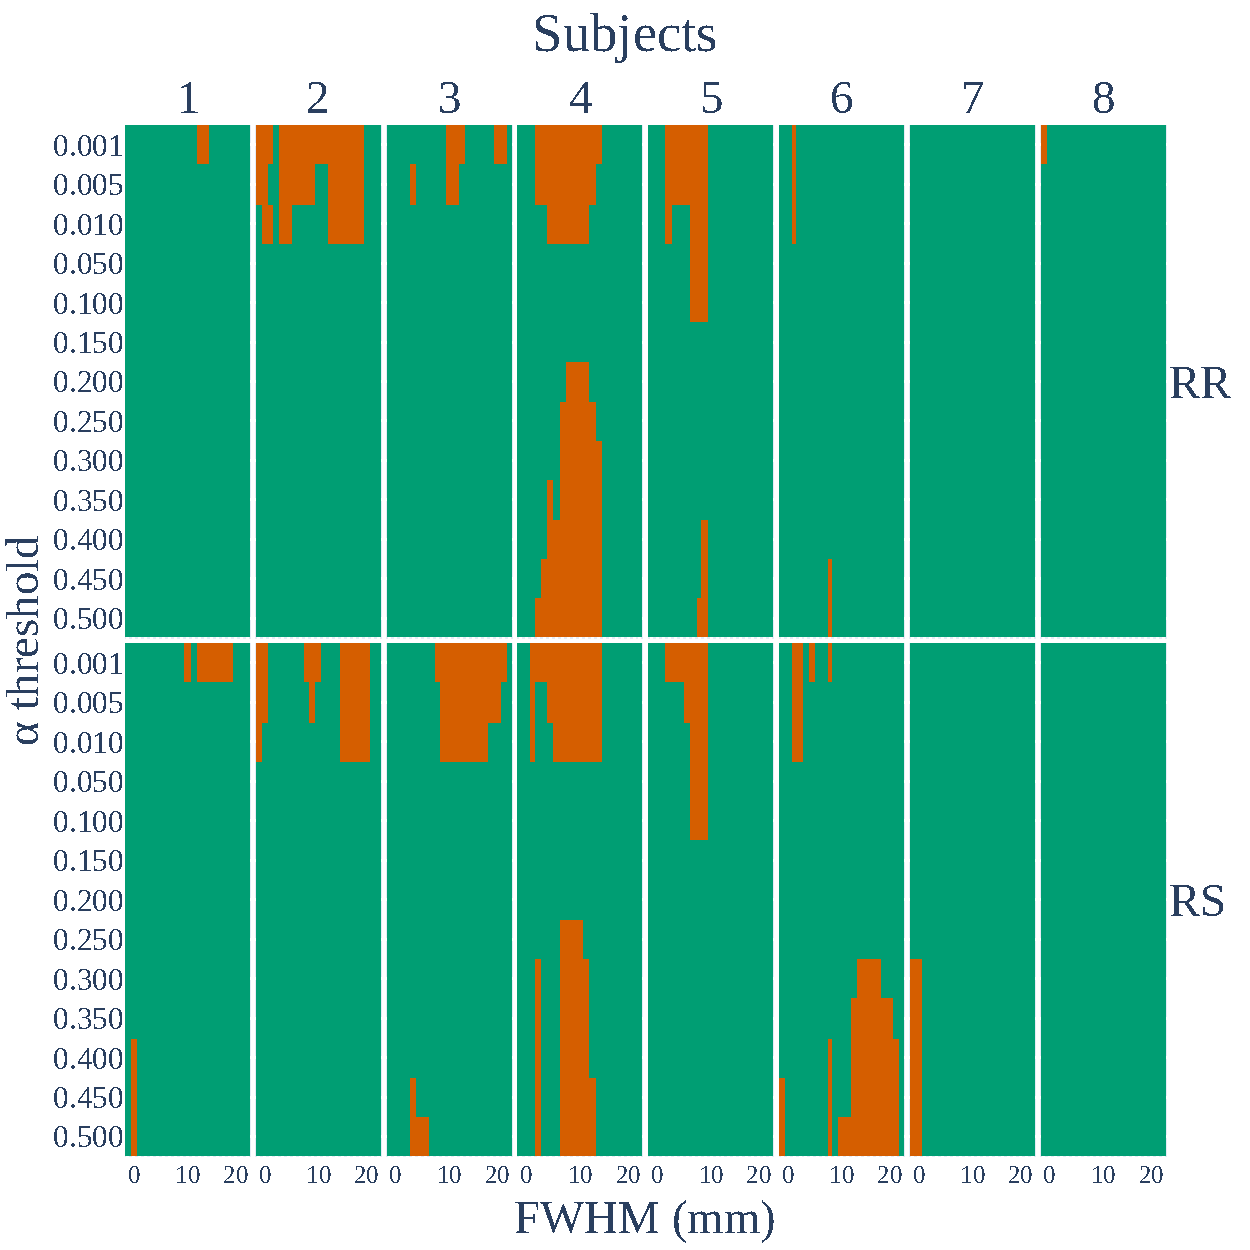
\includegraphics[width=\linewidth]{figures/loo_pce.pdf}
%     \caption{PCE}
%     \label{fig:loo_pce}
% \end{figure}

% \begin{figure}
%     \centering
%     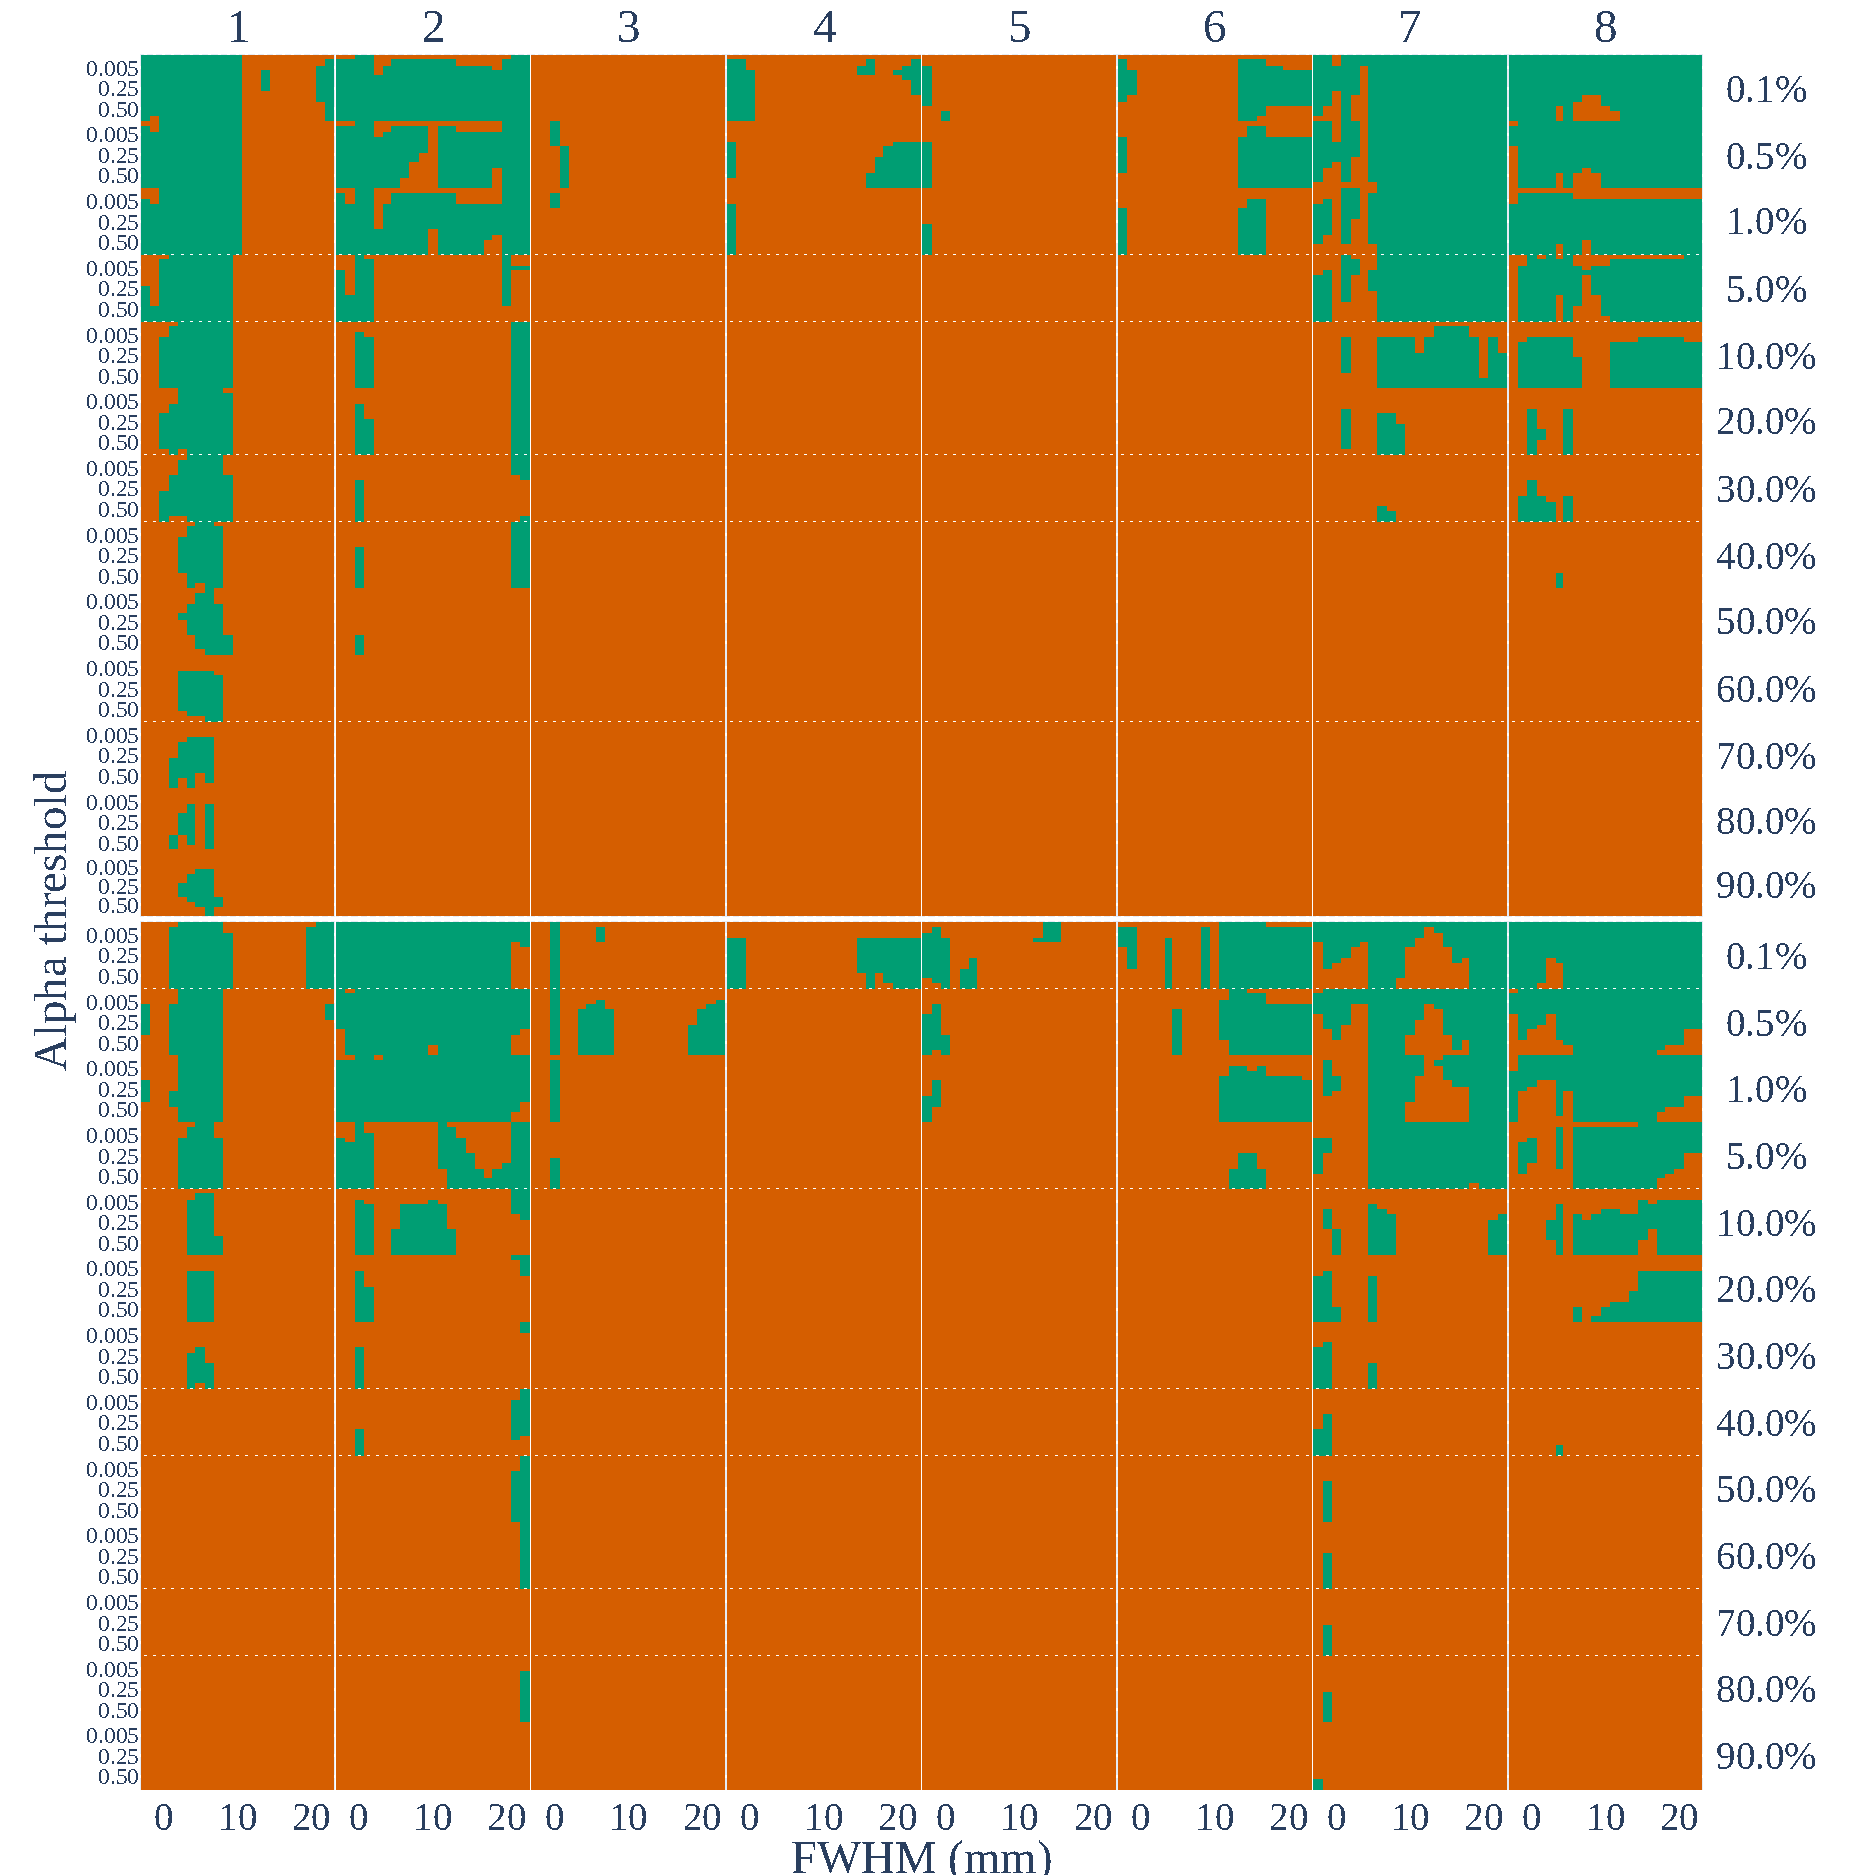
\includegraphics[width=\linewidth]{figures/template/template_pce.pdf}
%     \caption{Corrupted template check for RR and RS modes (pce)}
% \end{figure}


\end{document}

